% ============================================================================
% Chapter 3: The Lung Adenocarcinoma Use Case — Histopathology,
%            Molecular Landscape, Datasets, and Artefact Vision
% Thesis: Pattern-Informed Fuzzy Deep Learning for Interpretable
%         Genotype–Phenotype Inference in Lung Adenocarcinoma
%         under Data Scarcity
% Author: Servio F. Lima
% University of Fribourg
% ============================================================================

\chapter{The Lung Adenocarcinoma Use Case}
\label{ch:usecase}

This chapter introduces the cancer use case that motivates and grounds the computational artefacts developed in this thesis.
Following the Design Science Research methodology outlined in Section~\ref{sec:bg:dsr}, the use case serves a dual purpose: it defines the real-world problem to be addressed and it specifies the evaluation context in which the proposed artefacts must demonstrate their utility.

In contrast to Chapter~\ref{ch:background}, which presents the theoretical computational foundations, this chapter concentrates the histopathological and oncological domain knowledge required to interpret the clinical significance of the computational results.
Medical terms are explained at first use; a compact glossary is provided in Section~\ref{sec:uc:glossary} and a more comprehensive version in Appendix~\ref{app:glossary}.

The chapter proceeds as follows.
Section~\ref{sec:uc:clinical_problem} formulates the clinical problem in terms accessible to both engineering and medical readers.
Section~\ref{sec:uc:luad_histology} presents the six ANORAK-annotated histological growth patterns of LUAD (five WHO predominant patterns plus cribriform)---the microscopic ``building blocks'' that a pathologist uses to describe a tumour.
Section~\ref{sec:uc:molecular_landscape} describes the molecular landscape of LUAD: which genes are mutated, how those mutations shape what the tumour looks like under the microscope, and which drugs are available for each mutation.
All of this information is consolidated in a single reference table (Table~\ref{tab:gene_unified}) that links each gene to its morphology, biology, and treatment options.
Section~\ref{sec:uc:datasets} describes the datasets used for training and evaluation.
Section~\ref{sec:uc:data_scarcity} analyses the data scarcity challenge.
Section~\ref{sec:uc:clinical_questions} maps the seven research questions of Chapter~\ref{ch:introduction} onto the use case.
Section~\ref{sec:uc:pipeline_fixes} reports the headline figure of the pattern-classifier pipeline audit.
Section~\ref{sec:uc:artifact_vision} presents the vision for the three computational artefacts and the LCHAI~v2.0 prototype.
Finally, Section~\ref{sec:uc:experimental_design} states the headline of the six-condition benchmark, deferring the formal ablation logic and per-RQ comparisons to Chapter~\ref{ch:methodology}.


% ============================================================================
\section{The Clinical Problem}
\label{sec:uc:clinical_problem}
% ============================================================================

\paragraph{Problem statement.}
The prediction task addressed in this thesis is a multi-label binary
classification problem with bag-level supervision.
\textbf{Input}: one whole-slide image (WSI) per patient---a
gigapixel H\&E-stained tissue scan ($\sim 10^9$--$10^{10}$ pixels)
that the preprocessing pipeline partitions into
$N_s \in [\,5\,000,\, 80\,000\,]$ non-overlapping
$224 \times 224$ RGB tiles at $20\times$ magnification.
\textbf{Output}: a six-dimensional binary label vector
$\mathbf{y}_s \in \{0,1\}^6$, one bit per target gene
$g \in \mathcal{G} = \{\textit{TP53},\allowbreak\, \textit{EGFR},\allowbreak\, \textit{KRAS},\allowbreak\, \textit{STK11},\allowbreak\, \textit{KEAP1},\allowbreak\, \textit{RBM10}\}$,
indicating whether the slide's patient carries a non-silent somatic
mutation in that gene.
\textbf{Supervision} is \emph{bag-level}: each slide carries one
binary label \emph{per gene} (six labels in total), and a single
slide may be positive for several genes simultaneously---co-mutations
such as \textit{TP53}\,+\,\textit{KRAS} and
\textit{STK11}\,+\,\textit{KEAP1} are well documented in
LUAD~\cite{tcga2014luad,skoulidis2018stk11pd1}.
No tile-level mutation annotations exist, so the model must learn
which tiles within each slide carry the relevant morphological
evidence for each gene.
The remainder of this section explains the clinical motivation;
the artefacts that solve the task are presented in
Chapter~\ref{ch:methodology}.

\bigskip

When a patient is diagnosed with lung adenocarcinoma (LUAD), two categories of information guide treatment decisions (Figure~\ref{fig:luad_two_pillars})~\cite{herbst2018lung}.

\begin{figure}[ht!]
    \centering
    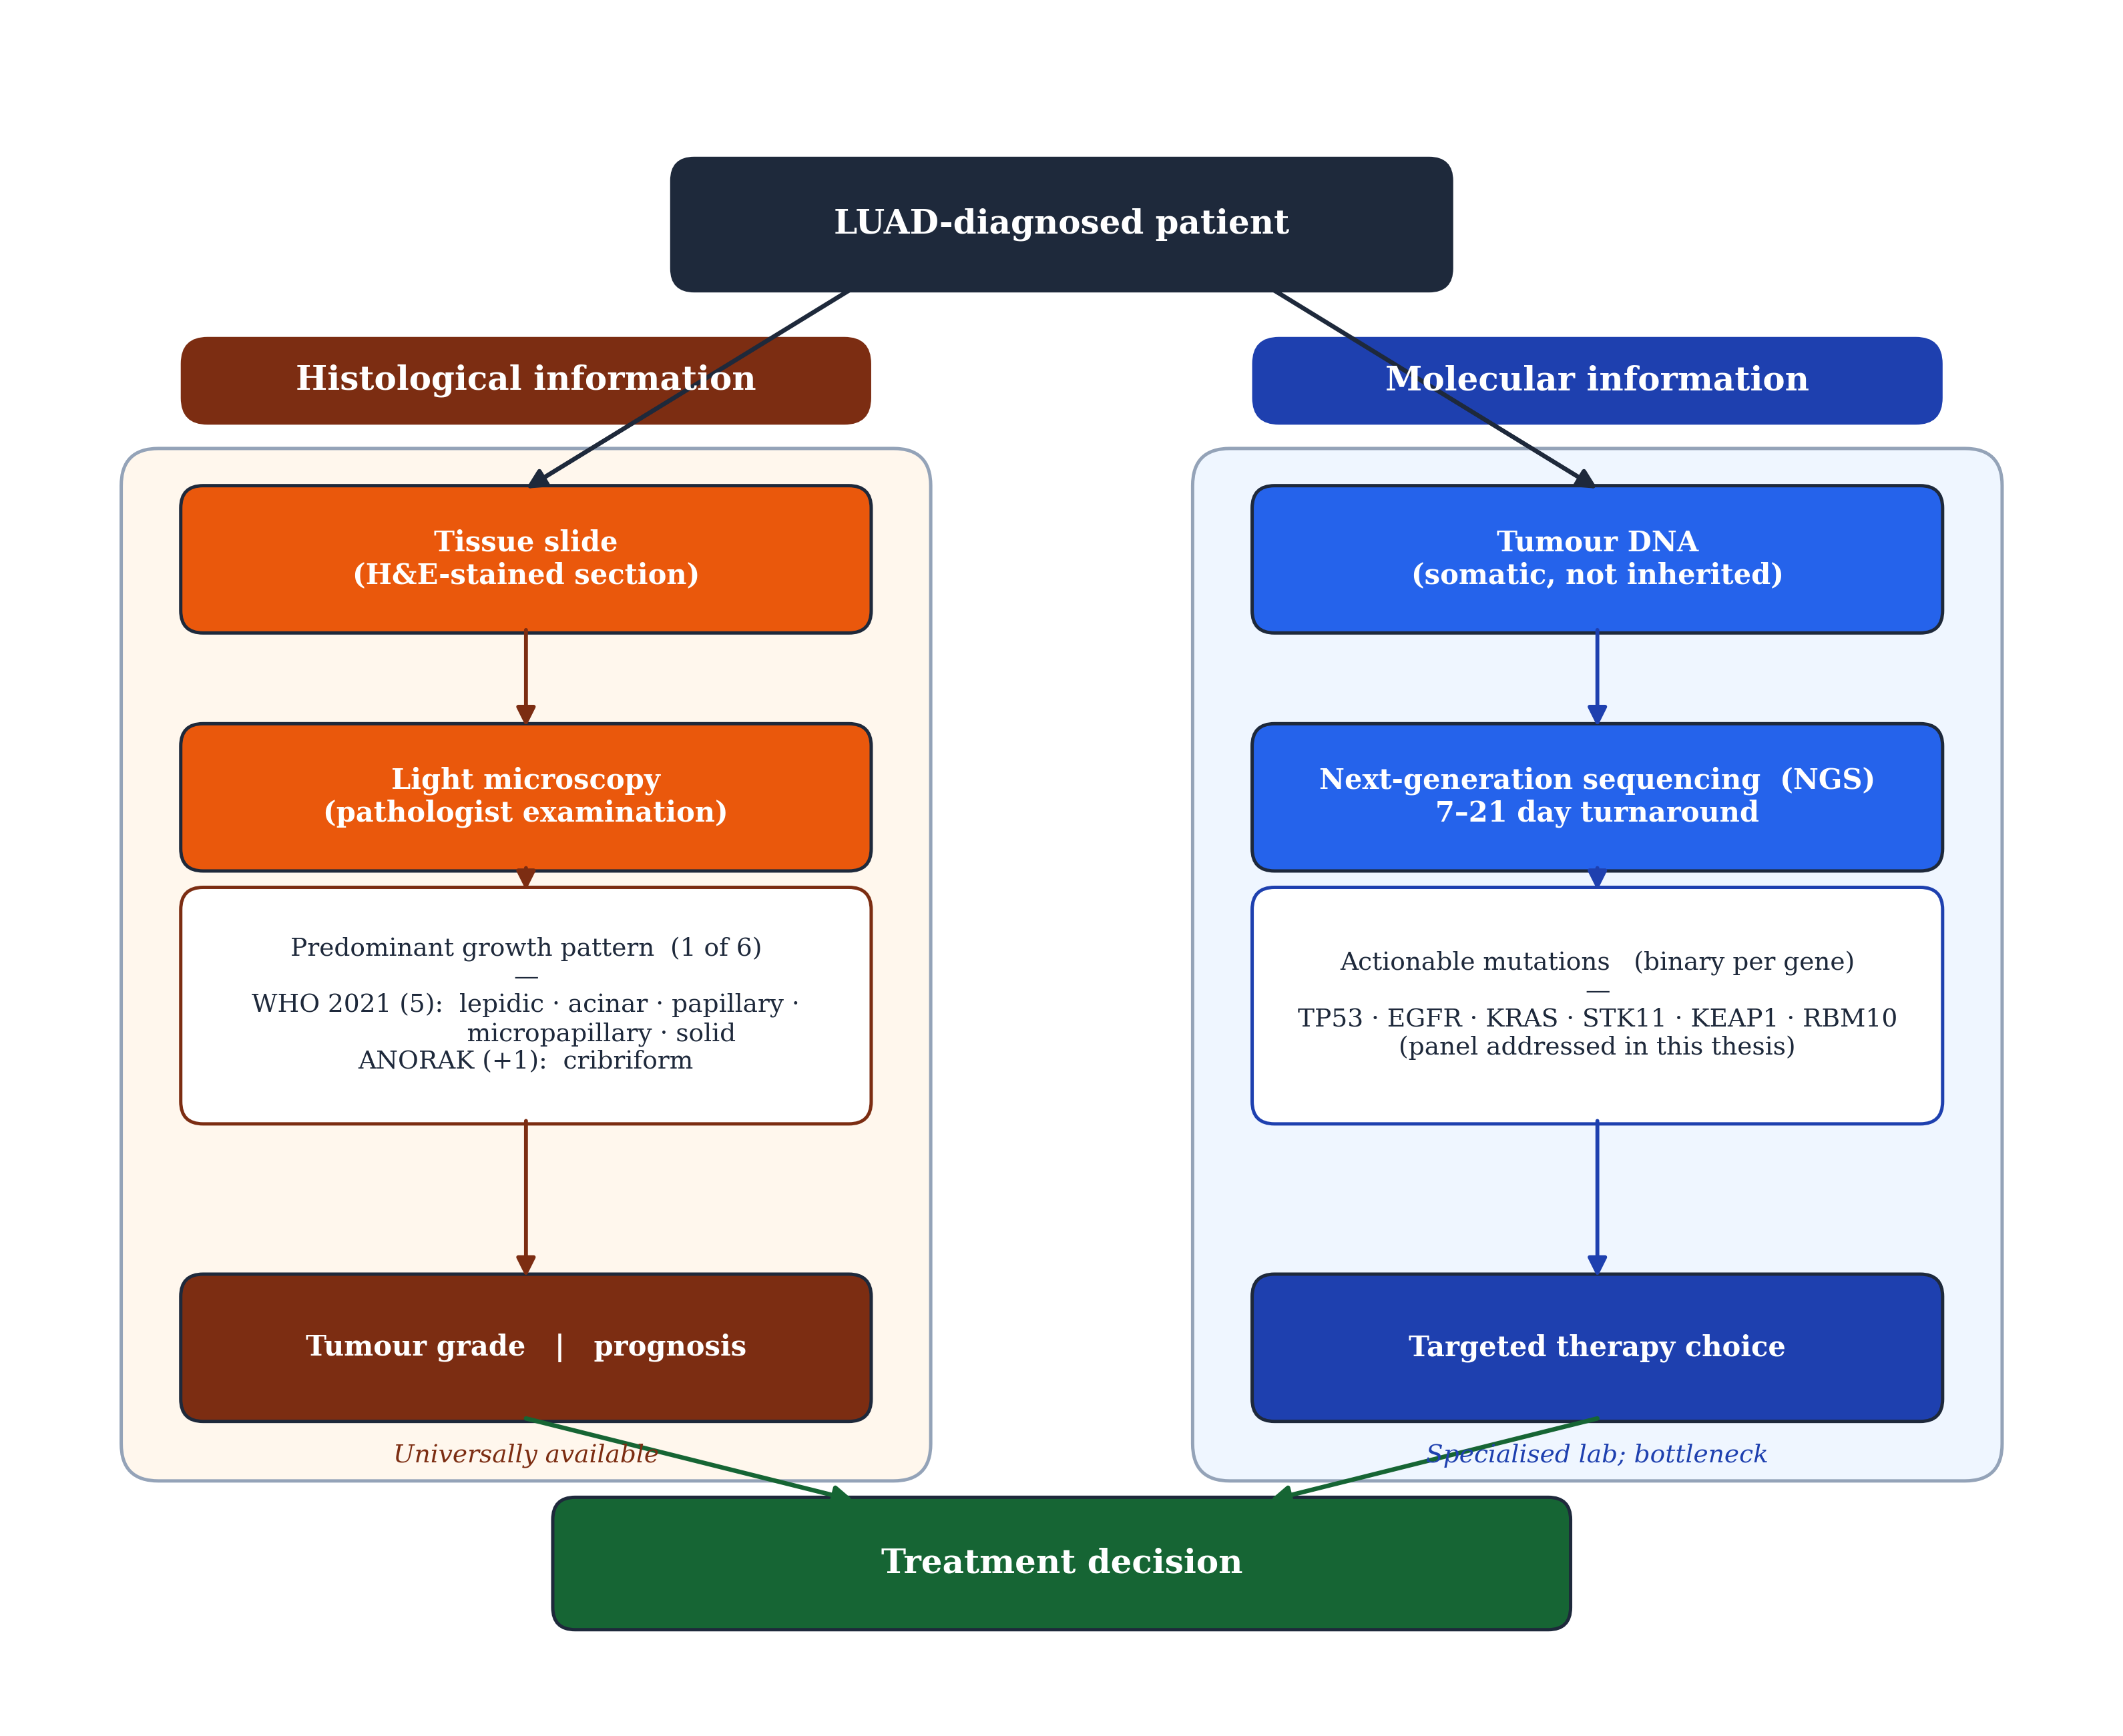
\includegraphics[width=0.92\textwidth]{chapters/figures/luad_two_pillars.png}
    \caption[Two pillars of LUAD diagnostic information]{%
        The two parallel categories of information that guide
        LUAD treatment decisions.
        \emph{Histological pillar (left):} an H\&E-stained tissue slide
        is examined under light microscopy and assigned a predominant
        growth pattern out of six labels (the five WHO 2021 patterns
        plus the ANORAK cribriform label adopted in this thesis);
        the predominant pattern determines tumour grade and prognosis.
        \emph{Molecular pillar (right):} tumour DNA is profiled by
        next-generation sequencing (NGS, 7--21 day turnaround) to
        produce a binary mutation status per gene over the panel
        $\mathcal{G} = \{\textit{TP53},\allowbreak\, \textit{EGFR},\allowbreak\, \textit{KRAS},\allowbreak\, \textit{STK11},\allowbreak\, \textit{KEAP1},\allowbreak\, \textit{RBM10}\}$ addressed in
        this thesis;
        the mutation profile drives the choice of targeted therapy.
        Both pillars feed the same downstream decision; the asymmetry
        in availability (microscopy is universal, NGS is the
        bottleneck) is the operational gap that motivates the
        prediction problem of this thesis.}
    \label{fig:luad_two_pillars}
\end{figure}

The first is \emph{histological}---what the tumour looks like under a microscope after staining a thin tissue slice with haematoxylin and eosin (H\&E), the universal stain that colours cell nuclei blue-purple and surrounding tissue pink.
A pathologist examines this stained slide and identifies the predominant growth pattern out of six labels (defined morphologically in Section~\ref{sec:uc:luad_histology}, Table~\ref{tab:luad_patterns}): five WHO-recognised patterns~\cite{who2021thoracic} plus cribriform, the additional label introduced by the ANORAK annotation guideline used by this thesis (Section~\ref{sec:uc:zenodo}). Together these six labels constitute the prediction target of Artefact~1; the pattern label determines the tumour's grade and carries prognostic significance.
The second category is \emph{molecular}---which genes carry somatic mutations (genetic changes acquired by the tumour, not inherited).
Molecular profiling is performed through next-generation sequencing (NGS), a laboratory technology that reads the DNA of tumour cells to identify mutations in clinically actionable genes such as \textit{TP53}, \textit{EGFR}, and \textit{KRAS}~\cite{tcga2014luad}.

\textbf{The bottleneck.}
While histological analysis is available wherever a pathologist and a microscope (or digital scanner) exist, molecular profiling requires specialised laboratory infrastructure, trained personnel, and consumables that are not universally accessible.
Turnaround times for NGS range from 7 to 21 days even at major European and North American centres~\cite{vanderlaan2018molecular}, creating a critical delay between biopsy and treatment initiation during which patients cannot receive targeted therapy.
In resource-limited settings---including many hospitals in Latin America, Africa, and Southeast Asia~\cite{sung2021global}---molecular profiling may not be available at all, making the need for rapid, slide-based mutation screening even more acute.
Yet treatment decisions depend critically on knowing the mutation status.
For example, a patient whose tumour carries an \textit{EGFR} mutation benefits dramatically from targeted drugs called tyrosine kinase inhibitors (TKIs); receiving standard chemotherapy instead of a TKI leads to a significantly worse outcome~\cite{soria2018flaura}.

\textbf{The opportunity.}
A growing body of evidence~\cite{coudray2018classification,kather2020pancancer} (reviewed in Section~\ref{sec:uc:molecular_landscape}) shows that certain mutations leave visible ``footprints'' in the H\&E slide---subtle but detectable changes in how the tumour cells arrange themselves.
If a computational system could read these footprints, it could provide a \emph{preliminary mutation prediction} directly from the histological slide, without waiting for NGS.
Such a prediction would not replace molecular profiling but could serve five purposes:
\begin{enumerate}
    \item \textbf{Triage:} Prioritise patients most likely to harbour actionable mutations for expedited NGS testing.
    \item \textbf{Preliminary guidance:} Inform initial treatment decisions while awaiting NGS results.
    \item \textbf{Access:} Provide mutation estimates in settings where NGS is unavailable, enabling referral to specialised centres.
    \item \textbf{Medical education:} The interpretability overlay (pattern maps, attention heatmaps, SHAP decompositions) provides an interactive tool for residents learning morphology--genotype relationships.
    \item \textbf{Research framework:} The architecture (fuzzy margin classification + pattern-informed MIL + Choquet aggregation + knowledge graph) is transferable to other cancer types with WHO-defined growth pattern taxonomies.
\end{enumerate}

\textbf{The interpretability requirement.}
For a mutation prediction to be clinically useful, a pathologist must be able to assess its plausibility.
A system that outputs ``TP53 mutated, probability 0.83'' without explanation provides no mechanism for clinical validation.
In contrast, a system that states ``TP53 likely mutated because the model attends to solid-enriched subregions ($3\times$ background prevalence), consistent with the high-grade dedifferentiation patterns known to be associated with TP53 mutation (which inactivates the tumour suppressor protein p53, leading to uncontrolled cell proliferation)'' allows the pathologist to examine those specific regions on the slide and judge whether the reasoning is sound.
This requirement for \emph{explainable mutation prediction} motivates the pattern-informed approach developed in this thesis.


\subsection{Glossary of Medical Terms}
\label{sec:uc:glossary}

Table~\ref{tab:glossary} provides definitions of the medical terms used throughout this thesis.
A more comprehensive glossary is provided in Appendix~\ref{app:glossary}.

\begin{table}[ht!]
\centering
\small
\caption{Glossary of essential medical terms used in this thesis.}
\label{tab:glossary}
\begin{tabular}{p{3.8cm} p{9.2cm}}
\hline
\textbf{Term} & \textbf{Definition} \\
\hline
Adenocarcinoma & A malignant tumour arising from glandular epithelial cells. LUAD is adenocarcinoma of the lung. \\
Biopsy & A tissue sample removed from the body for microscopic examination. \\
Driver mutation & A somatic mutation that confers a growth advantage to the tumour cell and contributes to cancer progression, as opposed to a ``passenger'' mutation with no functional effect. \\
H\&E staining & Haematoxylin and eosin staining; the standard histological stain that colours nuclei blue-purple and cytoplasm/stroma pink. Virtually all diagnostic pathology begins with an H\&E slide. \\
Histology & The study of tissue microstructure under a microscope. \\
Morphology & The form and structure of cells and tissues as observed under a microscope. Two tumours with the same gene mutation may look different; two tumours that look alike may carry different mutations. This imperfect correspondence is the challenge addressed in this thesis. \\
Next-generation sequencing (NGS) & High-throughput DNA sequencing technology that identifies mutations across multiple genes simultaneously. The ``gold standard'' for molecular profiling, but expensive and slow. \\
NSCLC & Non-small-cell lung cancer; the broad category encompassing LUAD, LUSC (squamous cell carcinoma), and large-cell carcinoma ($\sim$85\% of lung cancers). \\
Oncogene & A gene that, when mutated or overexpressed, actively promotes tumour growth (e.g., \textit{EGFR}, \textit{KRAS}). Think of it as a ``stuck accelerator.'' \\
Somatic mutation & A genetic alteration acquired by a tumour cell during the patient's lifetime (not inherited from parents). \\
Targeted therapy & A drug designed to interfere with a specific molecular target (e.g., EGFR inhibitors for \textit{EGFR}-mutant tumours). More effective and less toxic than traditional chemotherapy for the right patients, but only works if the mutation is present. \\
TKI & Tyrosine kinase inhibitor; a class of targeted drugs that block growth factor receptor signalling. Examples: erlotinib, osimertinib (for EGFR), sotorasib (for KRAS~G12C). \\
Tumour suppressor & A gene that normally acts as a ``brake'' on cell growth; its loss or inactivation removes that brake and allows uncontrolled proliferation (e.g., \textit{TP53}, \textit{STK11}). \\
Whole-slide image (WSI) & A high-resolution digital scan of an entire glass histology slide, typically containing $10^9$--$10^{10}$ pixels---comparable in file size to a feature film. \\
Wild-type & The non-mutated (normal) form of a gene. A tumour that is ``wild-type for EGFR'' does \emph{not} carry an EGFR mutation. \\
\hline
\end{tabular}
\end{table}


% ============================================================================
\section{LUAD Histopathology: The Six Growth Patterns}
\label{sec:uc:luad_histology}
% ============================================================================

\paragraph{Label space.}
This section defines the \textbf{label space of Artefact~1}.
Each $224\times 224$ tile is assigned a fuzzy membership vector
$\mathbf{p}_i \in \Delta^5$ (the 5-simplex over six classes) over the
six LUAD growth patterns described below: lepidic, acinar, papillary,
micropapillary, solid, and cribriform.
The first five are the WHO 2021 predominant patterns; the sixth is
the ANORAK-specific cribriform label adopted in this thesis to match
the public expert annotations.
The remainder of this section gives the morphological definition
of each class; the six labels are taken to be fixed, internally
consistent, and individually identifiable from a
$224\times 224$ patch at $20\times$ magnification.

\bigskip

Lung adenocarcinoma (LUAD) is the most common histological subtype of non-small-cell lung cancer, accounting for approximately 40\% of all lung malignancies~\cite{who2021thoracic}.
Unlike squamous cell carcinoma (LUSC), which arises from the bronchial lining and looks very different under the microscope, LUAD originates from the glandular cells of the peripheral lung.
What makes LUAD particularly challenging---both for pathologists and for machine learning---is that it does not look the same in every patient, or even within the same tumour.
Instead, the tumour cells can arrange themselves in several distinct architectural patterns, each with its own prognostic significance.


\subsection{WHO-Defined Growth Patterns}
\label{sec:uc:luad:patterns}

The first five of the six labels enumerated above are the predominant architectural patterns defined by the 2021 WHO Classification of Thoracic Tumours~\cite{who2021thoracic,nicholson2022ialcslurp}.
Cribriform architecture is described in the same framework as a high-grade pattern associated with acinar differentiation rather than as a separate sixth predominant category in the five-pattern reporting scheme~\cite{who2021thoracic}; the ANORAK dataset nevertheless annotates cribriform as its own tile-level class~\cite{anorak2024} and this thesis adopts the ANORAK six-class scheme accordingly.
Invasive mucinous adenocarcinoma (IMA) is recognised as a distinct LUAD variant; it is \emph{not} one of the six ANORAK pattern classes used computationally in this thesis, but remains clinically relevant when interpreting mucinous morphology in the literature.

Table~\ref{tab:luad_patterns} summarises each pattern's morphology, grade, prognosis, and computational characteristics.
Two clinical terms used in the table merit definition:
\begin{itemize}
    \item \textbf{Grade} refers to how abnormal the tumour cells appear
    under the microscope.  \emph{Low-grade} tumours (lepidic) closely
    resemble normal tissue and grow slowly; \emph{high-grade} tumours
    (solid, micropapillary) are poorly differentiated---their cells look
    very different from normal cells and tend to grow and spread more
    aggressively.  The IASLC grading system~\cite{moreira2020ialcslurp}
    assigns grade 1 (low) to lepidic-predominant, grade 2 (intermediate)
    to acinar- and papillary-predominant, and grade 3 (high) to solid-
    and micropapillary-predominant tumours.
    \item \textbf{Prognosis} refers to the expected clinical outcome.
    \emph{Favourable} prognosis indicates better survival rates after
    treatment; \emph{poor} prognosis indicates higher risk of recurrence
    and lower survival.  The predominant growth pattern is one of the
    strongest prognostic factors in resected LUAD~\cite{who2021thoracic}.
\end{itemize}
A non-specialist can think of the six patterns as different ways the
cancer cells ``build'' their tissue: growing along existing walls
(lepidic), forming tubes (acinar), creating finger-like projections
(papillary), floating in clusters (micropapillary), growing in flat
sheets (solid), or forming sieve-like fused glands (cribriform).
Histological terms used in the pattern descriptions (e.g.,
\emph{neoplastic}, \emph{alveolar}, \emph{stromal}, \emph{acini},
\emph{fibrovascular}) are defined in the Glossary
(Appendix~\ref{app:glossary}).

\begin{table}[!htbp]
\centering
\footnotesize
\renewcommand{\arraystretch}{1.05}
\caption[The six LUAD histological growth patterns used in this thesis.]{The six LUAD histological growth patterns used in this thesis,
with their morphological description, grade, prognosis, and key
computational characteristics.
Grade and prognosis follow the 2021 WHO Classification of Thoracic
Tumours~\cite{who2021thoracic} and the IASLC grading
proposal~\cite{moreira2020ialcslurp}.}
\label{tab:luad_patterns}
\setlength{\tabcolsep}{4pt}
\begin{tabular}{@{}l p{3.4cm} c c p{4.1cm}@{}}
\hline
\textbf{Pattern} &
\textbf{Morphological description} &
\textbf{Grade} &
\textbf{Prognosis} &
\textbf{Computational characteristics} \\
\hline

Lepidic &
Neoplastic cells grow along pre-existing alveolar walls without stromal
invasion; ``wallpaper-like'' spread along intact alveolar septa;
architecture preserved &
Low &
Favourable &
Subtle texture; highest classification uncertainty; 69 of
$\approx$509 training tiles (86 of 637; 13.5\%); benefits most from adaptive fuzzy margins \\[4pt]

Acinar &
Tumour cells form glandular structures (acini) of varying size with
a central lumen &
Intermediate &
Intermediate &
Most frequent class in the ANORAK split used here (145 training;
181 of 637; 28.4\%); also common in surgical LUAD cohorts; moderate visual distinctiveness;
largest class overlap with lepidic at boundaries \\[4pt]

Papillary &
Neoplastic cells line fibrovascular cores projecting into airspaces;
finger-like or branching structures &
Intermediate &
Intermediate &
Fibrovascular cores visible at 20$\times$; 100 training tiles (125 of 637; 19.6\%);
enriched in \textit{EGFR}-mutant tumours in many cohorts; overlaps with micropapillary \\[4pt]

Micropapillary &
Small tumour cell clusters lacking fibrovascular cores; float in
alveolar spaces or form ring-like tufts &
High &
Poor &
High-grade feature; associated with \textit{TP53} mutations; visually
distinctive floating clusters; strong attention signal in ABMIL;
minority class (55 training; 69 of 637; 10.8\%; tied smallest with cribriform) \\[4pt]

Solid &
Tumour cells grow in sheets without glandular, papillary, or lepidic
architecture; mucin may be present &
High &
Poor &
85 training tiles (107 of 637; 16.8\%); visually distinctive; high-grade pattern
often discussed alongside \textit{TP53} and \textit{KRAS} genotype--phenotype links
in the literature \\[4pt]

Cribriform &
Back-to-back glandular fusion without intervening stroma, forming
sieve-like (cribriform) structures; classified as a morphological
variant of acinar by WHO 2021~\cite{who2021thoracic} but annotated
as a distinct class in the ANORAK dataset~\cite{anorak2024} &
High &
Poor &
Complex glandular architecture; overlaps with acinar at boundaries;
annotated as label~1 in Zenodo--ANORAK; minority class (55 training;
69 of 637; 10.8\%; tied smallest with micropapillary) \\

\hline
\end{tabular}
\end{table}

All six growth patterns used in this thesis are illustrated in
Figure~\ref{fig:who_patterns_examples}, using representative tiles
from the expert-annotated Zenodo--ANORAK dataset~\cite{anorak2024}.
Figure~\ref{fig:zenodo_overlays} shows the corresponding expert-annotated
colour-coded overlays, which served as spatial ground truth for the
pattern classifier (Artefact~1).

\begin{figure}[ht!]
  \centering
  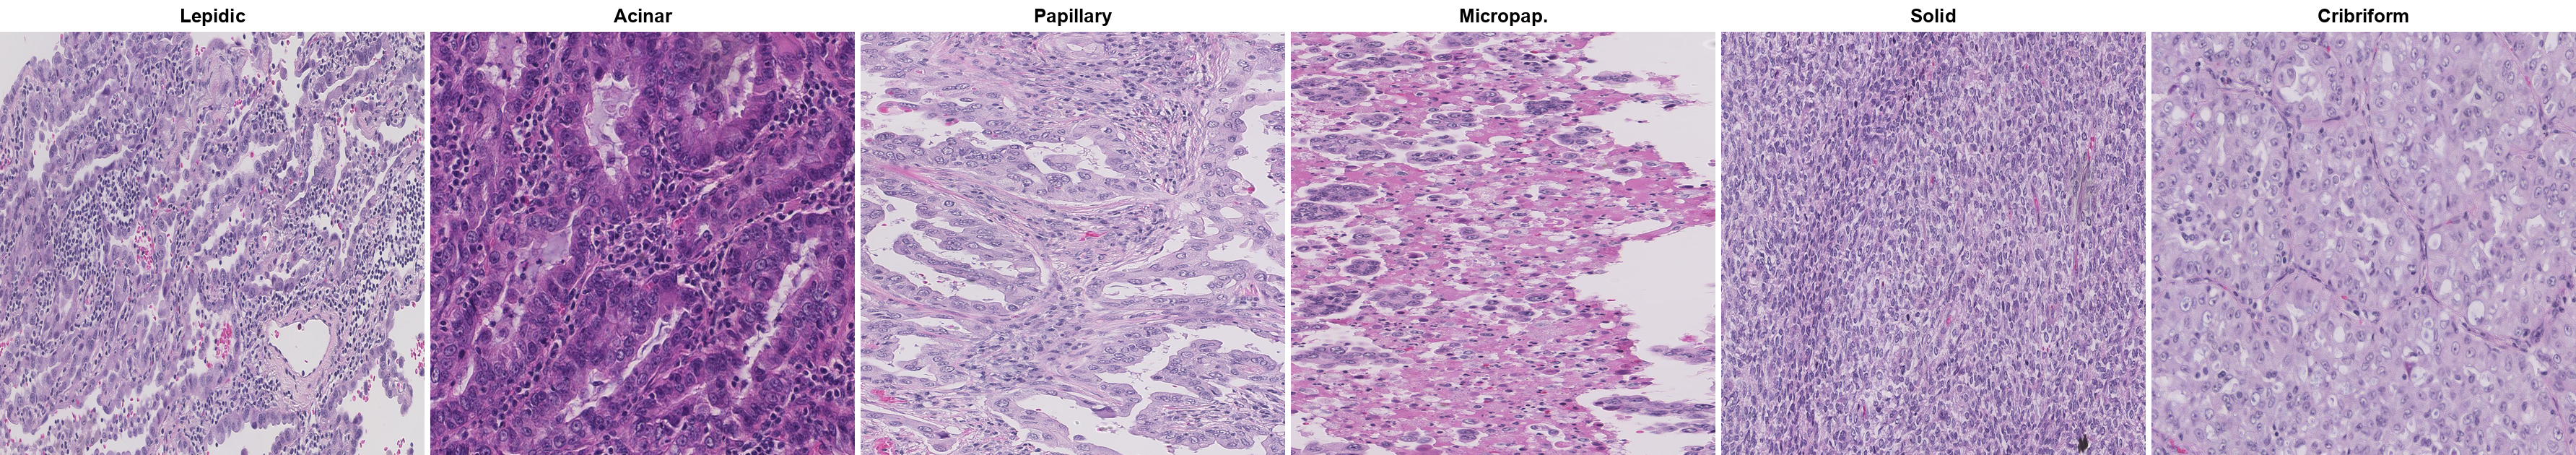
\includegraphics[width=\textwidth]{chapters/figures/who_luad_patterns.png}
  \caption[WHO/IASLC LUAD histological growth patterns]{%
      Representative H\&E-stained tiles for the six LUAD growth
      patterns used in this thesis, from the expert-annotated
      Zenodo--ANORAK dataset~\cite{anorak2024}.
      \textbf{Lepidic:} neoplastic cells growing along pre-existing
      alveolar walls without stromal invasion.
      \textbf{Acinar:} glandular structures with central lumina.
      \textbf{Papillary:} cells arranged on fibrovascular cores
      forming finger-like projections.
      \textbf{Micropapillary:} floating cell clusters lacking
      fibrovascular cores.
      \textbf{Solid:} sheet-like growth without glandular
      architecture.
      \textbf{Cribriform:} back-to-back glandular fusion without
      intervening stroma, forming sieve-like structures; classified
      as a high-grade acinar variant by WHO 2021~\cite{who2021thoracic}
      and annotated as a distinct class in the ANORAK
      dataset~\cite{anorak2024}.
      The five predominant patterns follow the 2021 WHO Classification
      of Thoracic Tumours~\cite{who2021thoracic}; cribriform is included
      as the sixth class following the ANORAK annotation scheme.}
  \label{fig:who_patterns_examples}
\end{figure}

\begin{figure}[ht!]
  \centering
  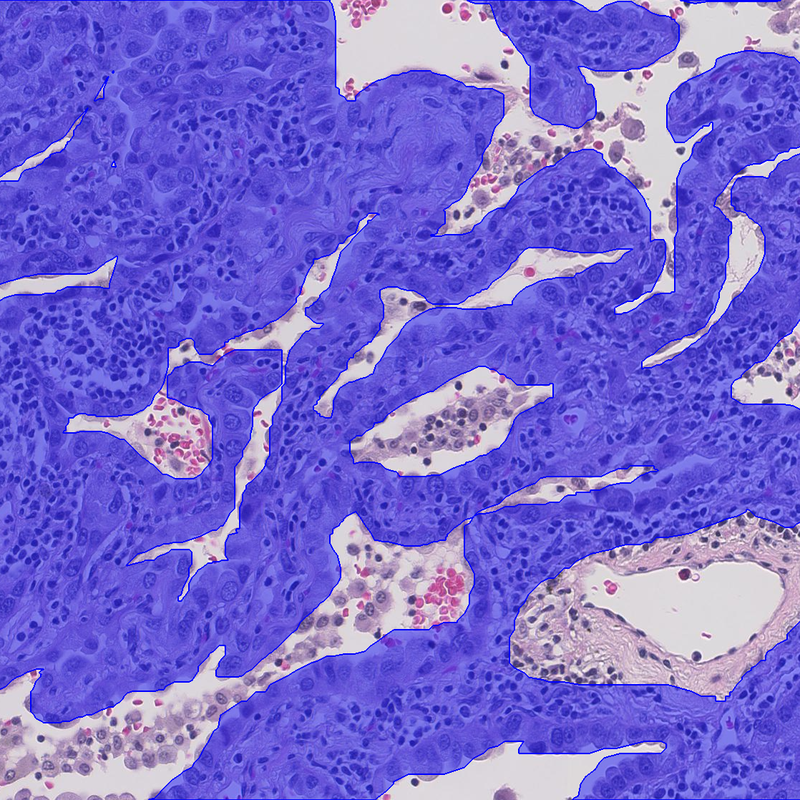
\includegraphics[width=0.155\textwidth]{chapters/figures/zenodo_overlay_lepidic.png}\hfill
  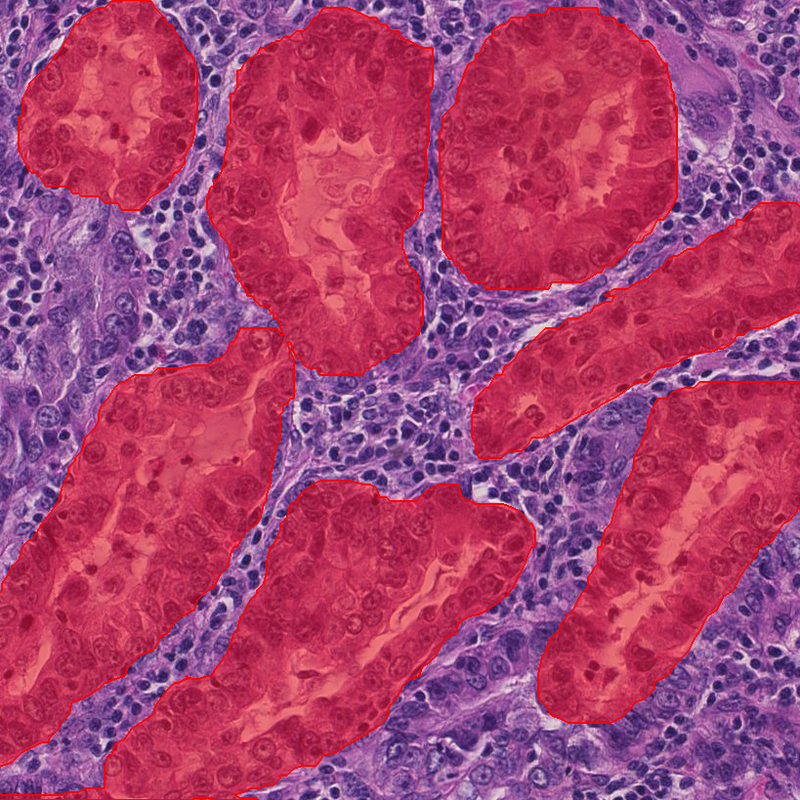
\includegraphics[width=0.155\textwidth]{chapters/figures/zenodo_overlay_acinar.png}\hfill
  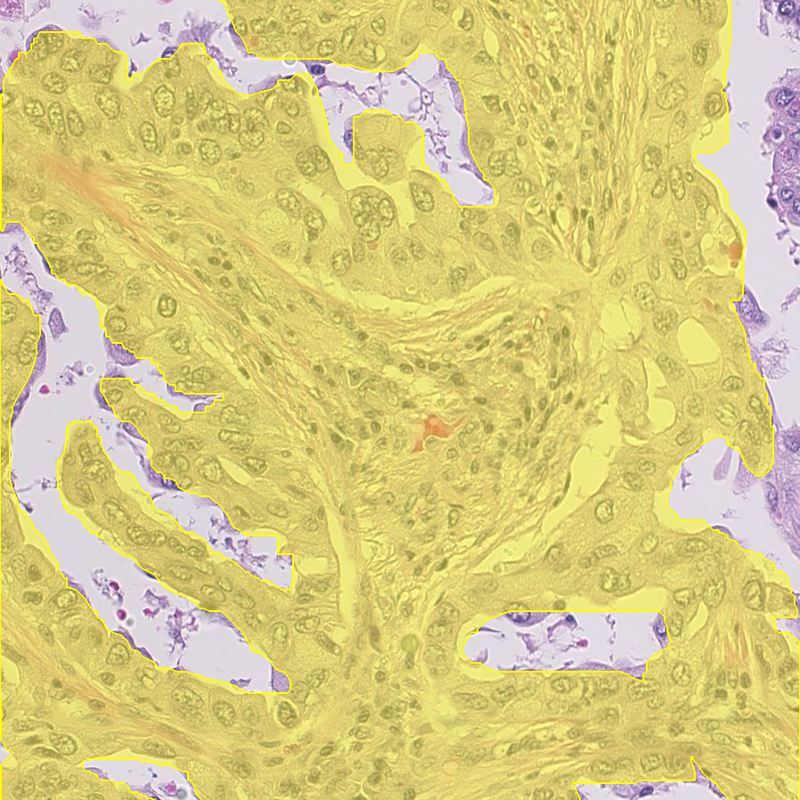
\includegraphics[width=0.155\textwidth]{chapters/figures/zenodo_overlay_papillary.png}\hfill
  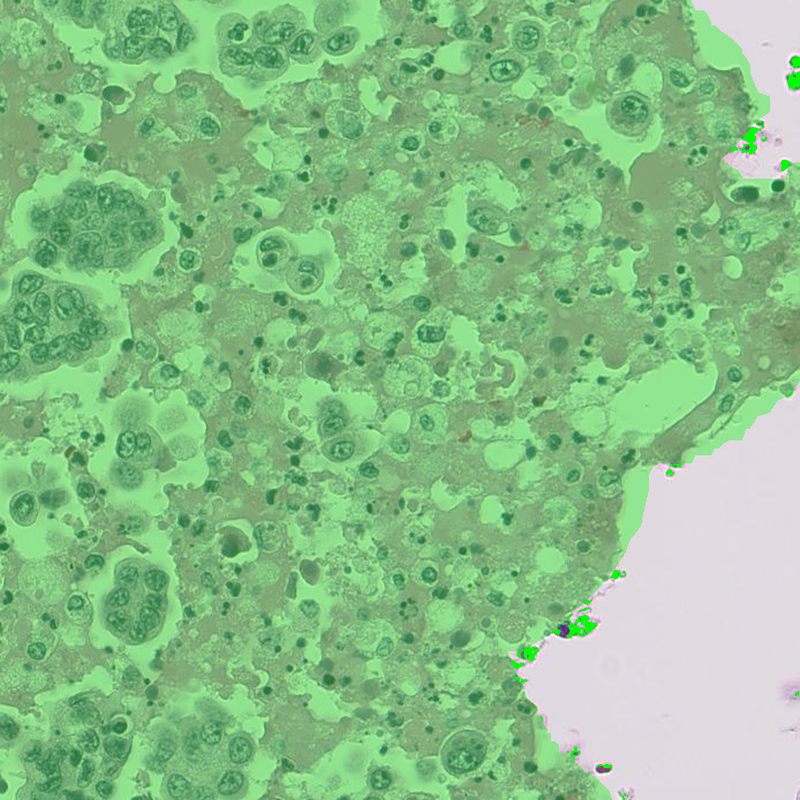
\includegraphics[width=0.155\textwidth]{chapters/figures/zenodo_overlay_micropapillary.png}\hfill
  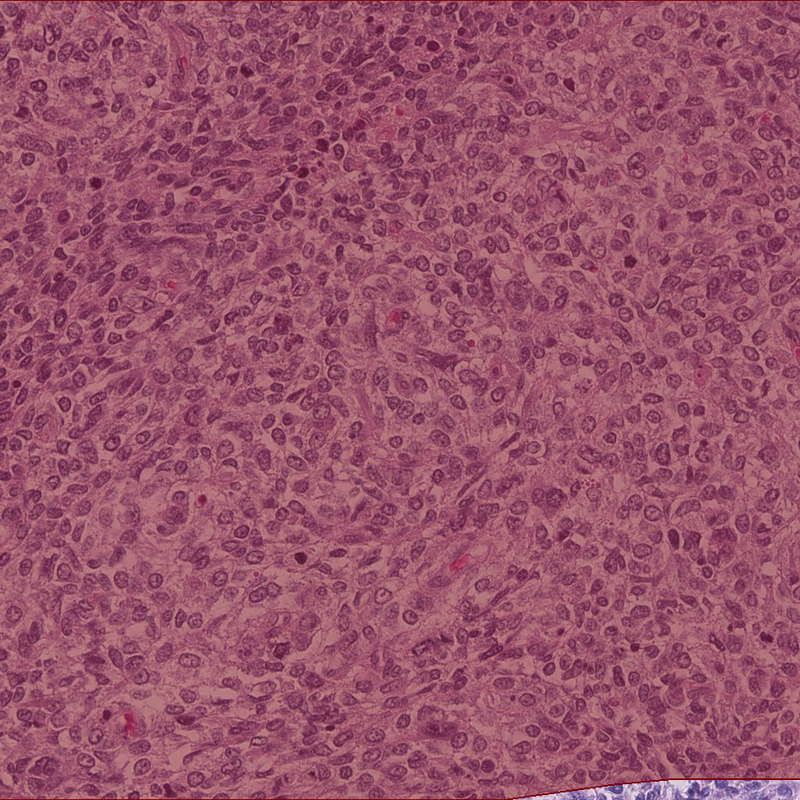
\includegraphics[width=0.155\textwidth]{chapters/figures/zenodo_overlay_solid.png}\hfill
  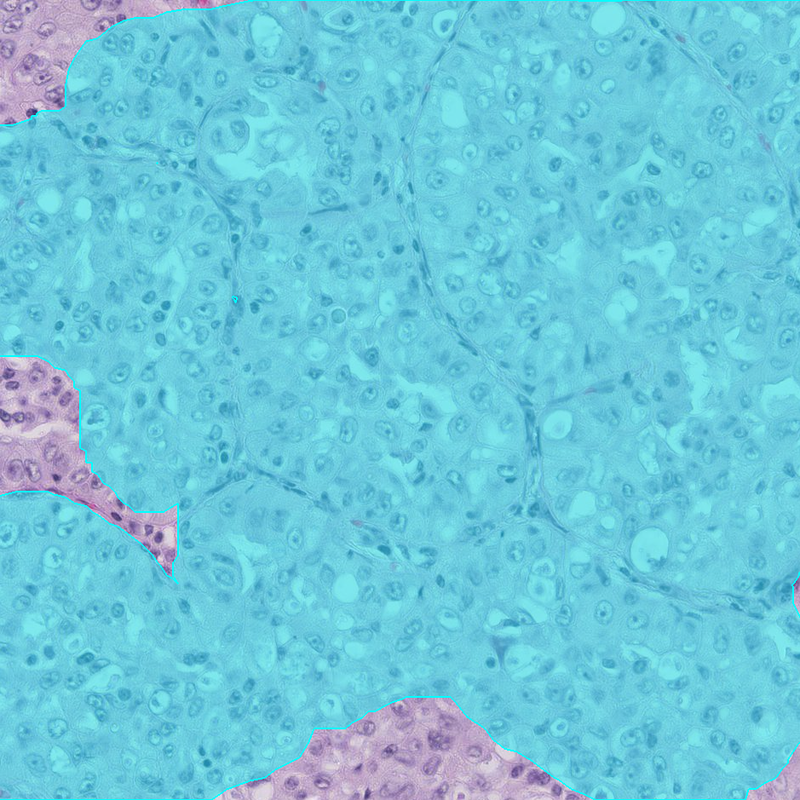
\includegraphics[width=0.155\textwidth]{chapters/figures/zenodo_overlay_cribriform.png}\\[2pt]
  {\small\hspace*{0.02\textwidth}%
  \makebox[0.155\textwidth]{\centering Lepidic}\hfill
  \makebox[0.155\textwidth]{\centering Acinar}\hfill
  \makebox[0.155\textwidth]{\centering Papillary}\hfill
  \makebox[0.155\textwidth]{\centering Micropap.}\hfill
  \makebox[0.155\textwidth]{\centering Solid}\hfill
  \makebox[0.155\textwidth]{\centering Cribriform}%
  \hspace*{0.02\textwidth}}
  \caption[Zenodo--ANORAK expert-annotated pattern overlays]{%
      Expert-annotated pattern overlays from the Zenodo--ANORAK
      dataset~\cite{anorak2024}, showing the colour-coded pathologist
      annotations superimposed on H\&E tiles.
      Each colour corresponds to one of the six ANORAK-annotated growth
      patterns used in this thesis: lepidic, acinar, papillary,
      micropapillary, solid, and cribriform.
      Of 732 raw images in the Zenodo repository, 637 tiles across 6
      classes were retained after excluding
      background/ambiguous (\emph{none}-class) tiles
      (Table~\ref{tab:dataset_config_anorak}).
      These overlays served as visual ground truth during model development,
      enabling direct comparison between model-predicted and expert-annotated
      spatial pattern distributions.}
  \label{fig:zenodo_overlays}
\end{figure}


\subsection{Intra-Tumoral Heterogeneity: Why One Tumour Contains Multiple Patterns}
\label{sec:uc:admixture}

A critical characteristic of LUAD---and the source of much of the
computational difficulty---is that most tumours do not consist of a
single, uniform pattern.
Instead, a typical resected LUAD specimen exhibits a mixture of two or
more patterns within the same slide~\cite{warth2012interobserver}.
The predominant pattern (the one occupying the largest area) determines
the histological grade, but even a small amount of a high-grade component
(solid or micropapillary) worsens the prognosis~\cite{moreira2020ialcslurp}.

In practice, patterns do not form cleanly separable compartments.
A region of acinar morphology may gradually transition into papillary
architecture over a few hundred micrometres, and transition zones
emerge where even expert pathologists disagree on the correct label.
The international interobserver study by Thunnissen
et~al.~\cite{thunnissen2012reproducibility}
quantified this phenomenon directly: across 26 expert thoracic
pathologists scoring the same set of LUAD cases, agreement on the
predominant growth pattern reached only $\kappa = 0.38$ (``fair'' on
the standard Landis--Koch scale), with the acinar--papillary boundary
being one of the most error-prone distinctions.
This $\kappa \approx 0.38$ figure is the empirical foundation for
treating the pattern label as inherently \emph{fuzzy} rather than
crisp---and therefore for the fuzzy-margin design of Artefact~1
(Section~\ref{sec:uc:artifact1}).
Figure~\ref{fig:growth_pattern_mapping} illustrates this phenomenon on a
representative LUAD specimen.

\begin{figure}[ht!]
  \centering
  \begin{minipage}[t]{0.48\textwidth}
  \centering
  \includegraphics[width=\textwidth]{chapters/figures/lchai_v2_KRAS_TCGA-55-7815_thumbnail.png}
  \end{minipage}\hfill
  \begin{minipage}[t]{0.48\textwidth}
  \centering
  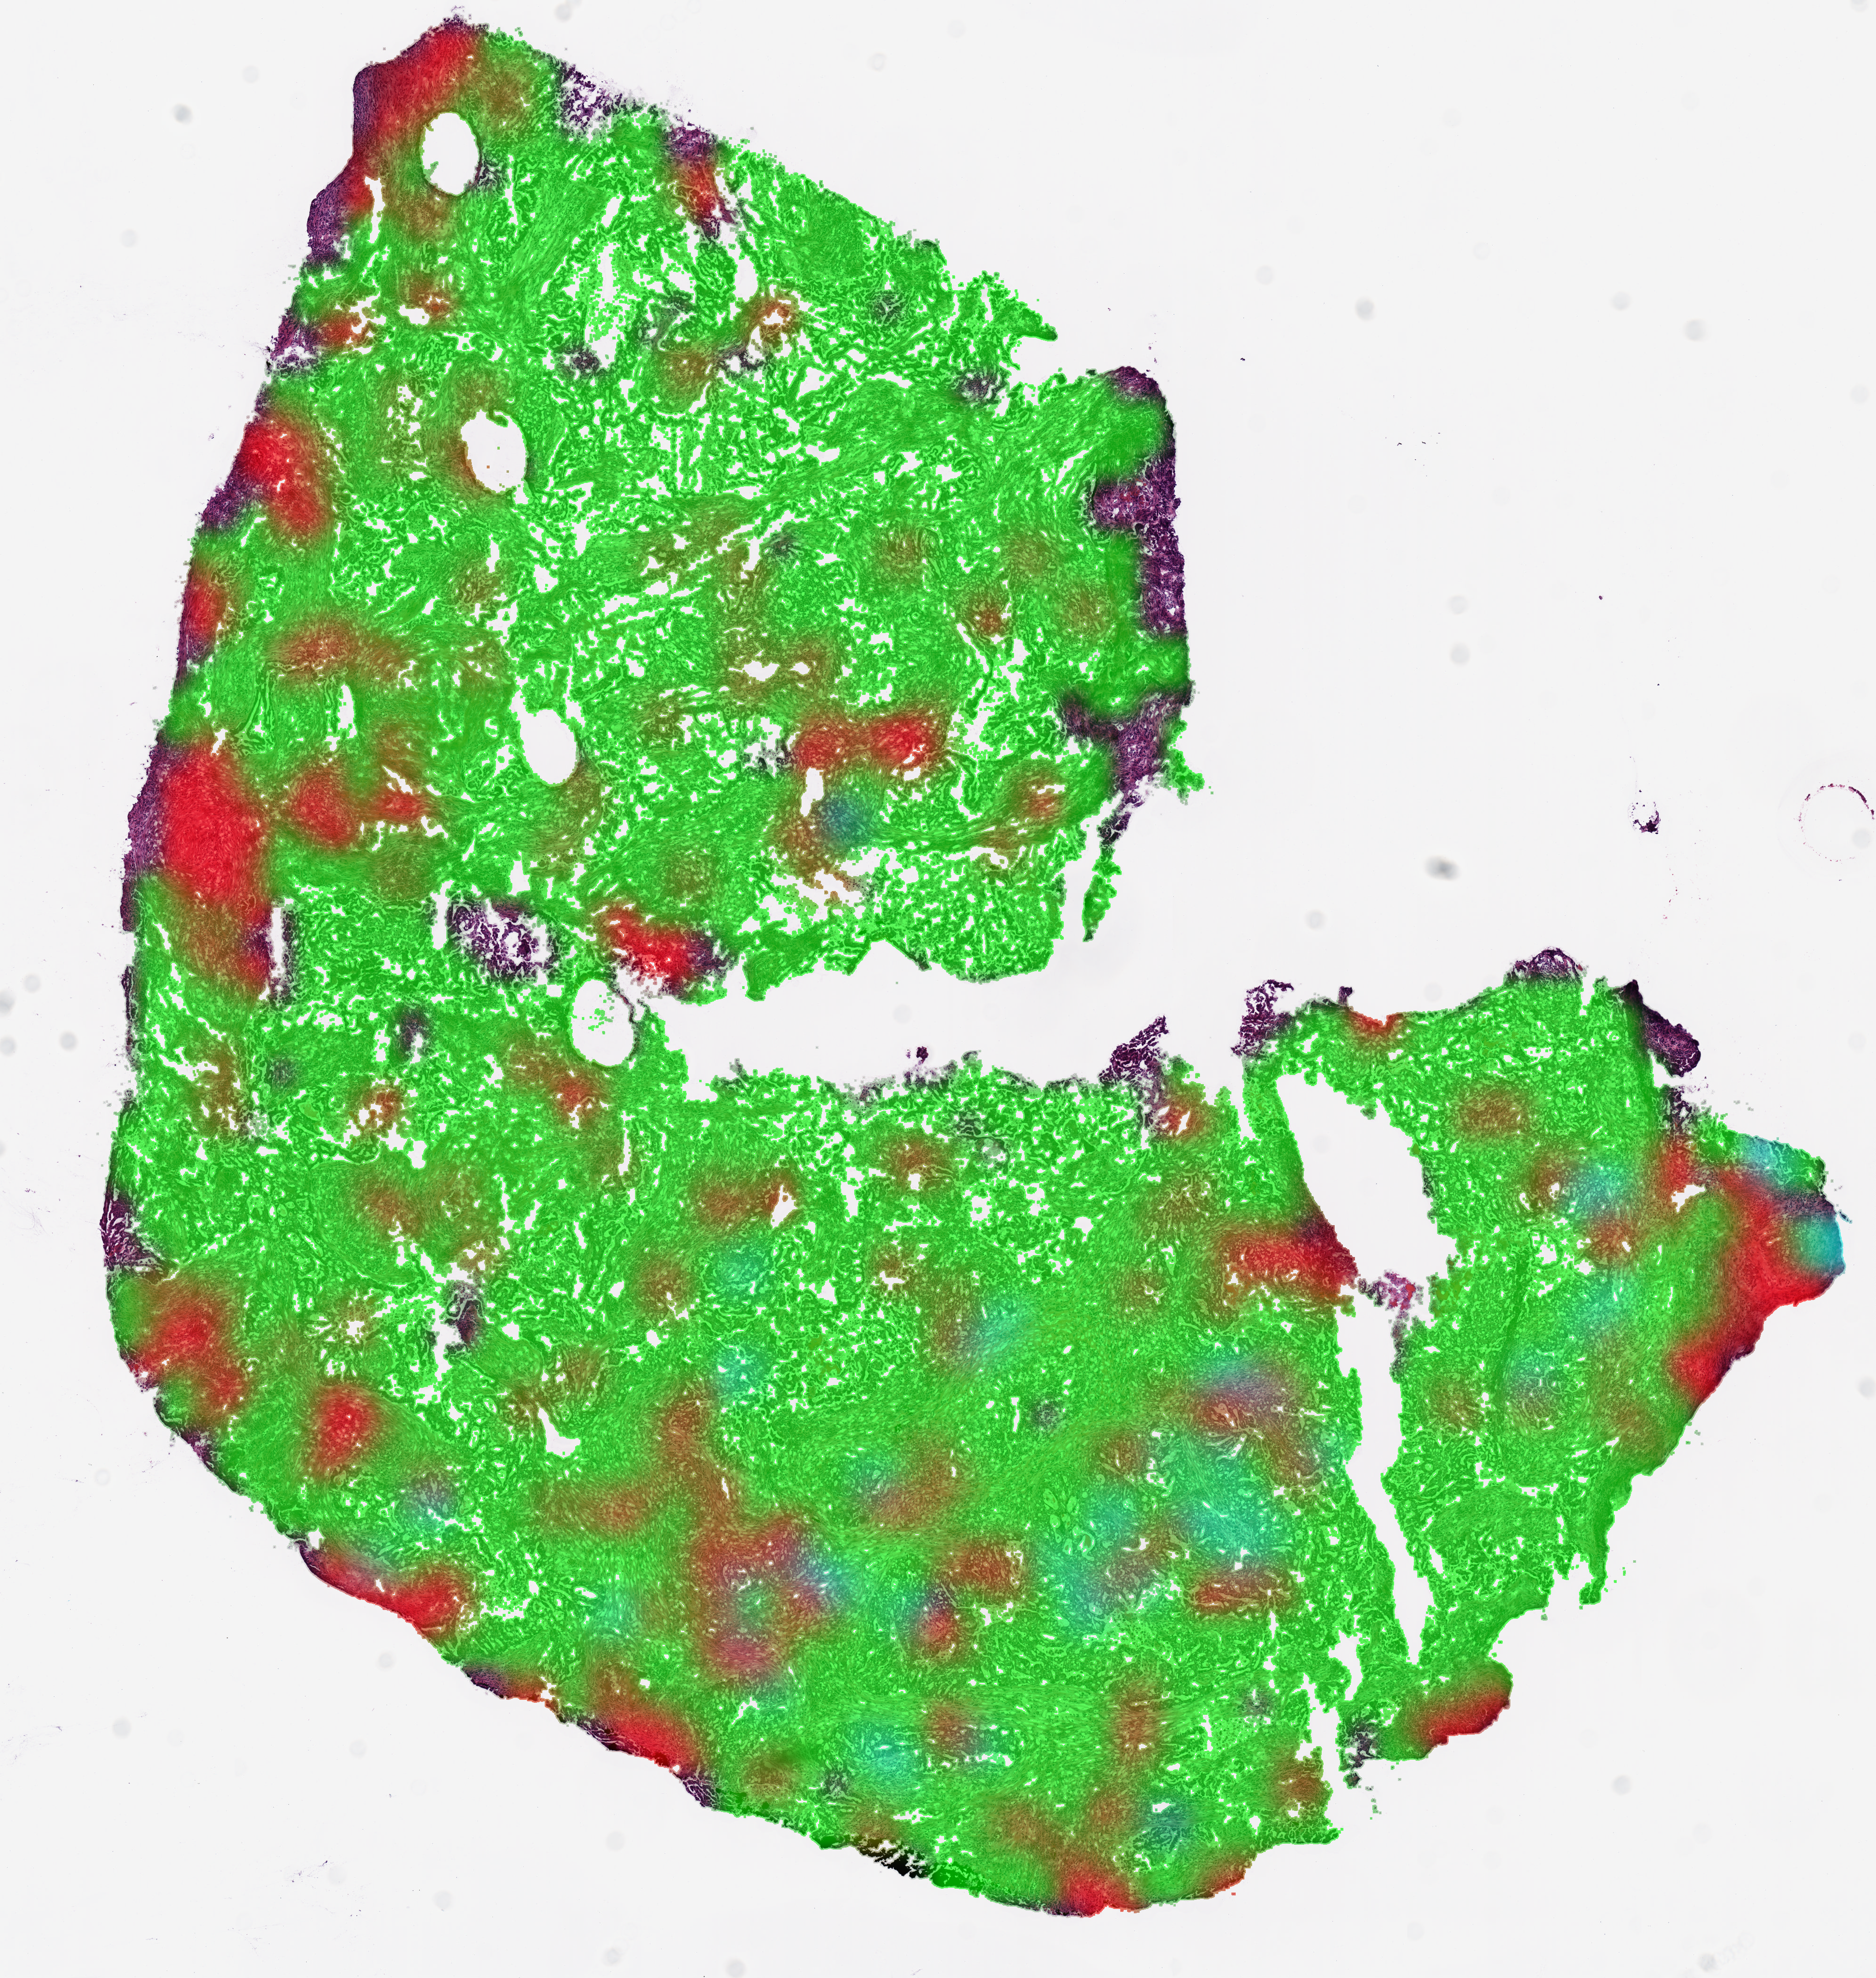
\includegraphics[width=\textwidth]{chapters/figures/lchai_v2_KRAS_TCGA-55-7815_pattern_overlay.png}
  \end{minipage}
  \caption[Spatial growth-pattern mapping in LUAD (TCGA-55-7815)]{%
      Spatial growth-pattern mapping for TCGA-55-7815, generated by
      LCHAI~v2.0 using the trained FuzzyArcLoss~V2 pattern classifier
      (Artefact~1).
      \textbf{Left:} original H\&E tissue section (1{,}708 tiles
      extracted at $224\times 224$ pixels).
      \textbf{Right:} tile-level pattern overlay with categorical
      colour coding: green~= micropapillary (79.4\%),
      red~= acinar (17.1\%), cyan~= cribriform (2.5\%),
      dark red~= solid (0.6\%), blue~= lepidic (0.2\%),
      yellow~= papillary (0.1\%).
      The overlay reveals that multiple architectural components
      co-occur spatially---acinar foci are interspersed within the
      dominant micropapillary background---and transition zones emerge
      where local tiles cannot be assigned unambiguously to a single
      class.
      This spatial admixture motivates both the fuzzy margin approach
      (FuzzyArcLoss~V2) and the interaction-aware aggregation
      (Fuzzy Choquet MIL).}
  \label{fig:growth_pattern_mapping}
\end{figure}

This spatial admixture has two direct consequences for the computational
approach of this thesis.
First, forcing a hard (yes/no) label onto each small image tile is
inherently lossy: it compresses a genuinely continuous morphological
spectrum into a single class.
This motivates FuzzyArcLoss~V2 (Section~\ref{sec:bg:fuzzy_margin}),
whose fuzzy membership function reduces harmful gradients on tiles at
morphological boundaries.
Second, because transition zones between patterns
(e.g.,~cribriform overlapping with acinar morphology, from which it
is derived---cribriform was historically grouped under acinar in the
WHO classification and was only later identified as a distinct
high-grade subset of acinar-predominant tumours by Kadota
et~al.~\cite{kadota2014cribriform})
make tile-level classification inherently ambiguous, the downstream
mutation inference stage must operate on case-level morphological
distributions rather than relying on any single tile's
classification---exactly the
regime where the Fuzzy Choquet aggregation
(Section~\ref{sec:bg:choquet}) provides its greatest benefit.


% ============================================================================
\section{Molecular Landscape: Mutations, Morphology, and Treatment}
\label{sec:uc:molecular_landscape}
% ============================================================================

\paragraph{Label space.}
This section defines the \textbf{label space of Artefact~2 and
Artefact~3}: a 6-dimensional binary mutation vector
$\mathbf{y}_s \in \{0,1\}^6$ over the gene panel
$\mathcal{G} = \{\textit{TP53},\allowbreak\, \textit{EGFR},\allowbreak\, \textit{KRAS},\allowbreak\, \textit{STK11},\allowbreak\, \textit{KEAP1},\allowbreak\, \textit{RBM10}\}$,
matching the canonical gene order used in Chapters~\ref{ch:methodology}
and~\ref{ch:evaluation} (Table~\ref{tab:gene_unified}).
For each gene the table also encodes an \emph{a priori expected
discrimination mode}: a per-gene prior over where the discriminative
signal is expected to live, expressed in five thesis-specific
organising labels, each grounded in an established concept:
\textsc{Direct (saturable)}---a single dominant pattern is the
discriminative signal and is therefore expected to be already absorbed
by a strong pretrained pathology encoder, leaving little headroom for
an explicit pattern channel~\cite{wang2022ctranspath,coudray2018classification};
\textsc{Interaction-driven}---the signal lives in pairwise pattern
co-occurrence (e.g.\ lepidic\,$\times$\,solid as a proxy for IMA)
and therefore requires a non-additive aggregator with explicit
interaction indices~\cite{grabisch2009aggregation};
\textsc{Off-modality (TME)}---the discriminative axis lies inside
H\&E but outside the 6-pattern ANORAK simplex, in the tumour
microenvironment (e.g.\ STK11's immune-cold
phenotype)~\cite{skoulidis2018stk11pd1};
\textsc{Off-modality (biochemical)}---the signal does not project
into the H\&E modality at all, residing in an upstream biochemical
regulator with no robust visible correlate (e.g.\ the KEAP1/NRF2
oxidative-stress pathway)~\cite{li2011keap1papillary,tcga2014luad};
and \textsc{Low-prevalence stress test}---the positive class is
small enough that no head can depart from the base-rate prior, the
canonical class-imbalance failure mode~\cite{lin2017focal}.
Chapter~\ref{ch:evaluation} (RQ2(ii)) recasts each gene's empirical
result into a separate but mappable taxonomy of three observed regimes
(\emph{Regime~A}: encoder-saturation; \emph{Regime~B}:
out-of-ontology, with three sub-mechanisms---label-space mismatch,
no morphological projection, and collapse-to-prior; \emph{Regime~C}:
cross-term in label space), so that each gene's a priori expectation
listed below can be matched against the empirical verdict
(Table~\ref{tab:rq_mapping}).

\bigskip

LUAD is among the most thoroughly characterised cancers at the molecular
level.
The Cancer Genome Atlas (TCGA) project---which has grown to
668 LUAD patients with paired WSIs and mutation
data~\cite{tcga2014luad}---identified recurrent driver mutations---genetic changes
that actively fuel the tumour's growth---in genes including
\textit{TP53}, \textit{EGFR}, \textit{KRAS}, \textit{STK11},
\textit{KEAP1}, and \textit{RBM10}~\cite{tcga2014luad}.
These mutations matter clinically because they determine which drugs will
work: a patient with an \textit{EGFR} mutation can receive a targeted
therapy---a tyrosine kinase inhibitor (TKI) such as
osimertinib~\cite{soria2018flaura}---that is far more effective than
traditional chemotherapy,
while a patient with a \textit{KRAS}~G12C mutation now has access to a
new class of targeted inhibitors (sotorasib,
adagrasib)~\cite{skoulidis2021codebreak} that were unavailable just
five years ago.

Crucially, these mutations are not invisible on the slide.
A growing body of evidence shows that certain driver mutations
reshape the tumour's microscopic architecture in statistically
predictable, heterogeneous ways.
The per-gene morphology--mutation associations relevant to this
thesis---together with the biology, the a priori discrimination
mode, the targeted therapy, and the supporting literature
citations---are summarised in Table~\ref{tab:gene_unified}.
These associations are the biological foundation of the entire
thesis: if an algorithm can recognise the histological patterns and
learn which pattern distributions are associated with which mutations,
it can bridge the gap between the microscope and molecular profiling.


\subsection{The Six Target Genes: An Integrated View}
\label{sec:uc:six_genes}

This thesis targets six genes for mutation prediction.
Table~\ref{tab:gene_unified} consolidates all gene-specific information
into a single integrated reference.
For each gene the table provides:
(i)~its prevalence $p_g = n_+/N$ in the 687-slide cohort;
(ii)~its functional class (TS = tumour suppressor, OG = oncogene,
RBP = RNA-binding protein);
(iii)~the morphological correlate reported in the literature;
(iv)~a one-line biology statement;
(v)~its \emph{a priori} expected discrimination mode---the prior
expectation about \emph{how} the signal (if any) is encoded in the
H\&E modality, expressed in the same vocabulary that
Chapter~\ref{ch:evaluation} uses to taxonomise the empirical regimes;
and (vi)~the targeted-therapy landscape in two lines.
The empirical verification of column~(v) is what
Chapter~\ref{ch:evaluation} reports.

\begin{table}[!htbp]
\centering
\footnotesize
\caption[Integrated per-gene reference for the 6-gene LUAD
panel.]{Integrated per-gene reference for the 6-gene panel
$\mathcal{G} = \{\textit{TP53},\allowbreak\, \textit{EGFR},\allowbreak\, \textit{KRAS},\allowbreak\, \textit{STK11},\allowbreak\, \textit{KEAP1},\allowbreak\, \textit{RBM10}\}$.
Rows are ordered by descending TCGA-LUAD prevalence
$p_g = n_+/N$ in the 687-slide cohort used in this thesis;
the canonical gene order used elsewhere in the thesis is
$(\textit{TP53},\allowbreak\, \textit{EGFR},\allowbreak\, \textit{KRAS},\allowbreak\, \textit{STK11},\allowbreak\, \textit{KEAP1},\allowbreak\, \textit{RBM10})$.
The \emph{a priori} expected discrimination mode column states the
prior expectation about how the morphological signal (if any) maps
into the 6-pattern ANORAK simplex
(\textsc{Direct/saturable}, \textsc{Interaction-driven},
\textsc{Off-modality (TME)}, \textsc{Off-modality (biochemical)},
\textsc{Low-prevalence stress test}); these priors are matched
against the empirical regimes of Chapter~\ref{ch:evaluation}
(Regime~A/B/C) in Table~\ref{tab:rq_mapping}.
Type abbreviations: TS = tumour suppressor, OG = oncogene,
RBP = RNA-binding protein.
Therapy column current as of 2025; reader is referred to current
NCCN guidelines for clinical decisions.
Citations for the morphology--mutation associations:
TP53~\cite{ahn2022tp53highgrade};
KRAS~\cite{shim2015krasmucinous,rekhtman2013krassolid};
KEAP1~\cite{li2011keap1papillary,tcga2014luad};
EGFR~\cite{yoshizawa2013egfrmorph};
STK11~\cite{skoulidis2015krassubsets};
RBM10~\cite{tcga2014luad}.}
\label{tab:gene_unified}
\resizebox{\textwidth}{!}{%
\begin{tabular}{@{} l r l p{2.6cm} p{2.6cm} l p{2.6cm} @{}}
\toprule
\textbf{Gene} &
\textbf{$p_g$} &
\textbf{Type} &
\textbf{Morph.\ correlate} &
\textbf{Biology (1-line)} &
\textbf{A priori mode} &
\textbf{Targeted therapy} \\
\midrule

\textit{TP53}  & 38.0\,\% & TS  &
Solid · micropapillary; nuclear pleomorphism, high-grade &
p53 loss $\Rightarrow$ cell-cycle brake released; dedifferentiation &
\textsc{Direct (saturable)} &
None targeted; IO if TMB high; chemotherapy standard
\\[3pt]

\textit{KRAS}  & 20.4\,\% & OG  &
IMA, solid, mucin-rich acinar; pale/foamy cytoplasm &
RAS/MAPK constitutively active; G12D enriched in IMA &
\textsc{Interaction-driven} (e.g.\ lepidic\,$\times$\,solid for IMA proxy) &
Sotorasib, adagrasib (G12C-only); MEK inhibitors in trials
\\[3pt]

\textit{KEAP1} & 14.3\,\% & TS  &
Weak; loose papillary association; no robust visible signature &
NRF2 antioxidant pathway; biochemical / metabolic effect &
\textsc{Off-modality (biochemical)} &
NRF2 pathway inhibitors (early trials); concurrent
\textit{KEAP1/STK11} predicts IO resistance
\\[3pt]

\textit{EGFR}  & 11.4\,\% & OG  &
Lepidic · papillary; low atypia, well-differentiated &
RTK growth signal; proliferation without genomic instability &
\textsc{Direct (saturable)} &
Osimertinib (1L, 3rd-gen TKI); erlotinib/gefitinib/afatinib;
T790M $\to$ sequential therapy
\\[3pt]

\textit{STK11} & 9.9\,\% & TS  &
No tumour-cell pattern; reduced TILs / immune-cold stroma in TME &
LKB1 inactivation $\Rightarrow$ immune-suppressive
microenvironment &
\textsc{Off-modality (TME)} &
None targeted; \emph{negative} IO biomarker (predicts resistance)
\\[3pt]

\textit{RBM10} & 5.4\,\% & RBP &
None established; $n_+ = 37$ (only 5.4\,\%) &
RNA splicing dysregulation; indirect/heterogeneous phenotype &
\textsc{Low-prevalence stress test} &
None approved; splicing modulators at research stage
\\

\bottomrule
\end{tabular}}
\begin{flushleft}
\scriptsize
\textsc{Direct (saturable)}: signal is read directly from a single
dominant pattern (or pair) and is therefore expected to be already
captured by a pretrained encoder such as CTransPath, leaving little
headroom for the explicit pattern channel.
\textsc{Interaction-driven}: signal lives in pairwise co-occurrence
of patterns (e.g.\ KRAS-driven invasive mucinous adenocarcinoma is
proxied by lepidic\,$\times$\,solid co-presence) and therefore
requires a non-additive aggregator (Choquet integral) rather than
concatenation.
\textsc{Off-modality (TME)}: discriminative direction lies outside
the 6-pattern ANORAK simplex but inside H\&E---specifically in the
tumour microenvironment (immune infiltrate density, stromal
texture).
\textsc{Off-modality (biochemical)}: signal does not project into
the H\&E modality at all---an upstream biochemical regulator with no
robust visible correlate.
\textsc{Low-prevalence stress test}: positive class $n_+$ small
enough that no head can depart from the base-rate prior.
Abbreviations: IMA = invasive mucinous adenocarcinoma;
RTK = receptor tyrosine kinase;
TIL = tumour-infiltrating lymphocyte;
TME = tumour microenvironment;
TMB = tumour mutation burden;
IO = immunotherapy (anti-PD-1 / anti-PD-L1);
TKI = tyrosine kinase inhibitor;
1L = first-line.
\end{flushleft}
\end{table}

\begin{figure}[ht!]
    \centering
    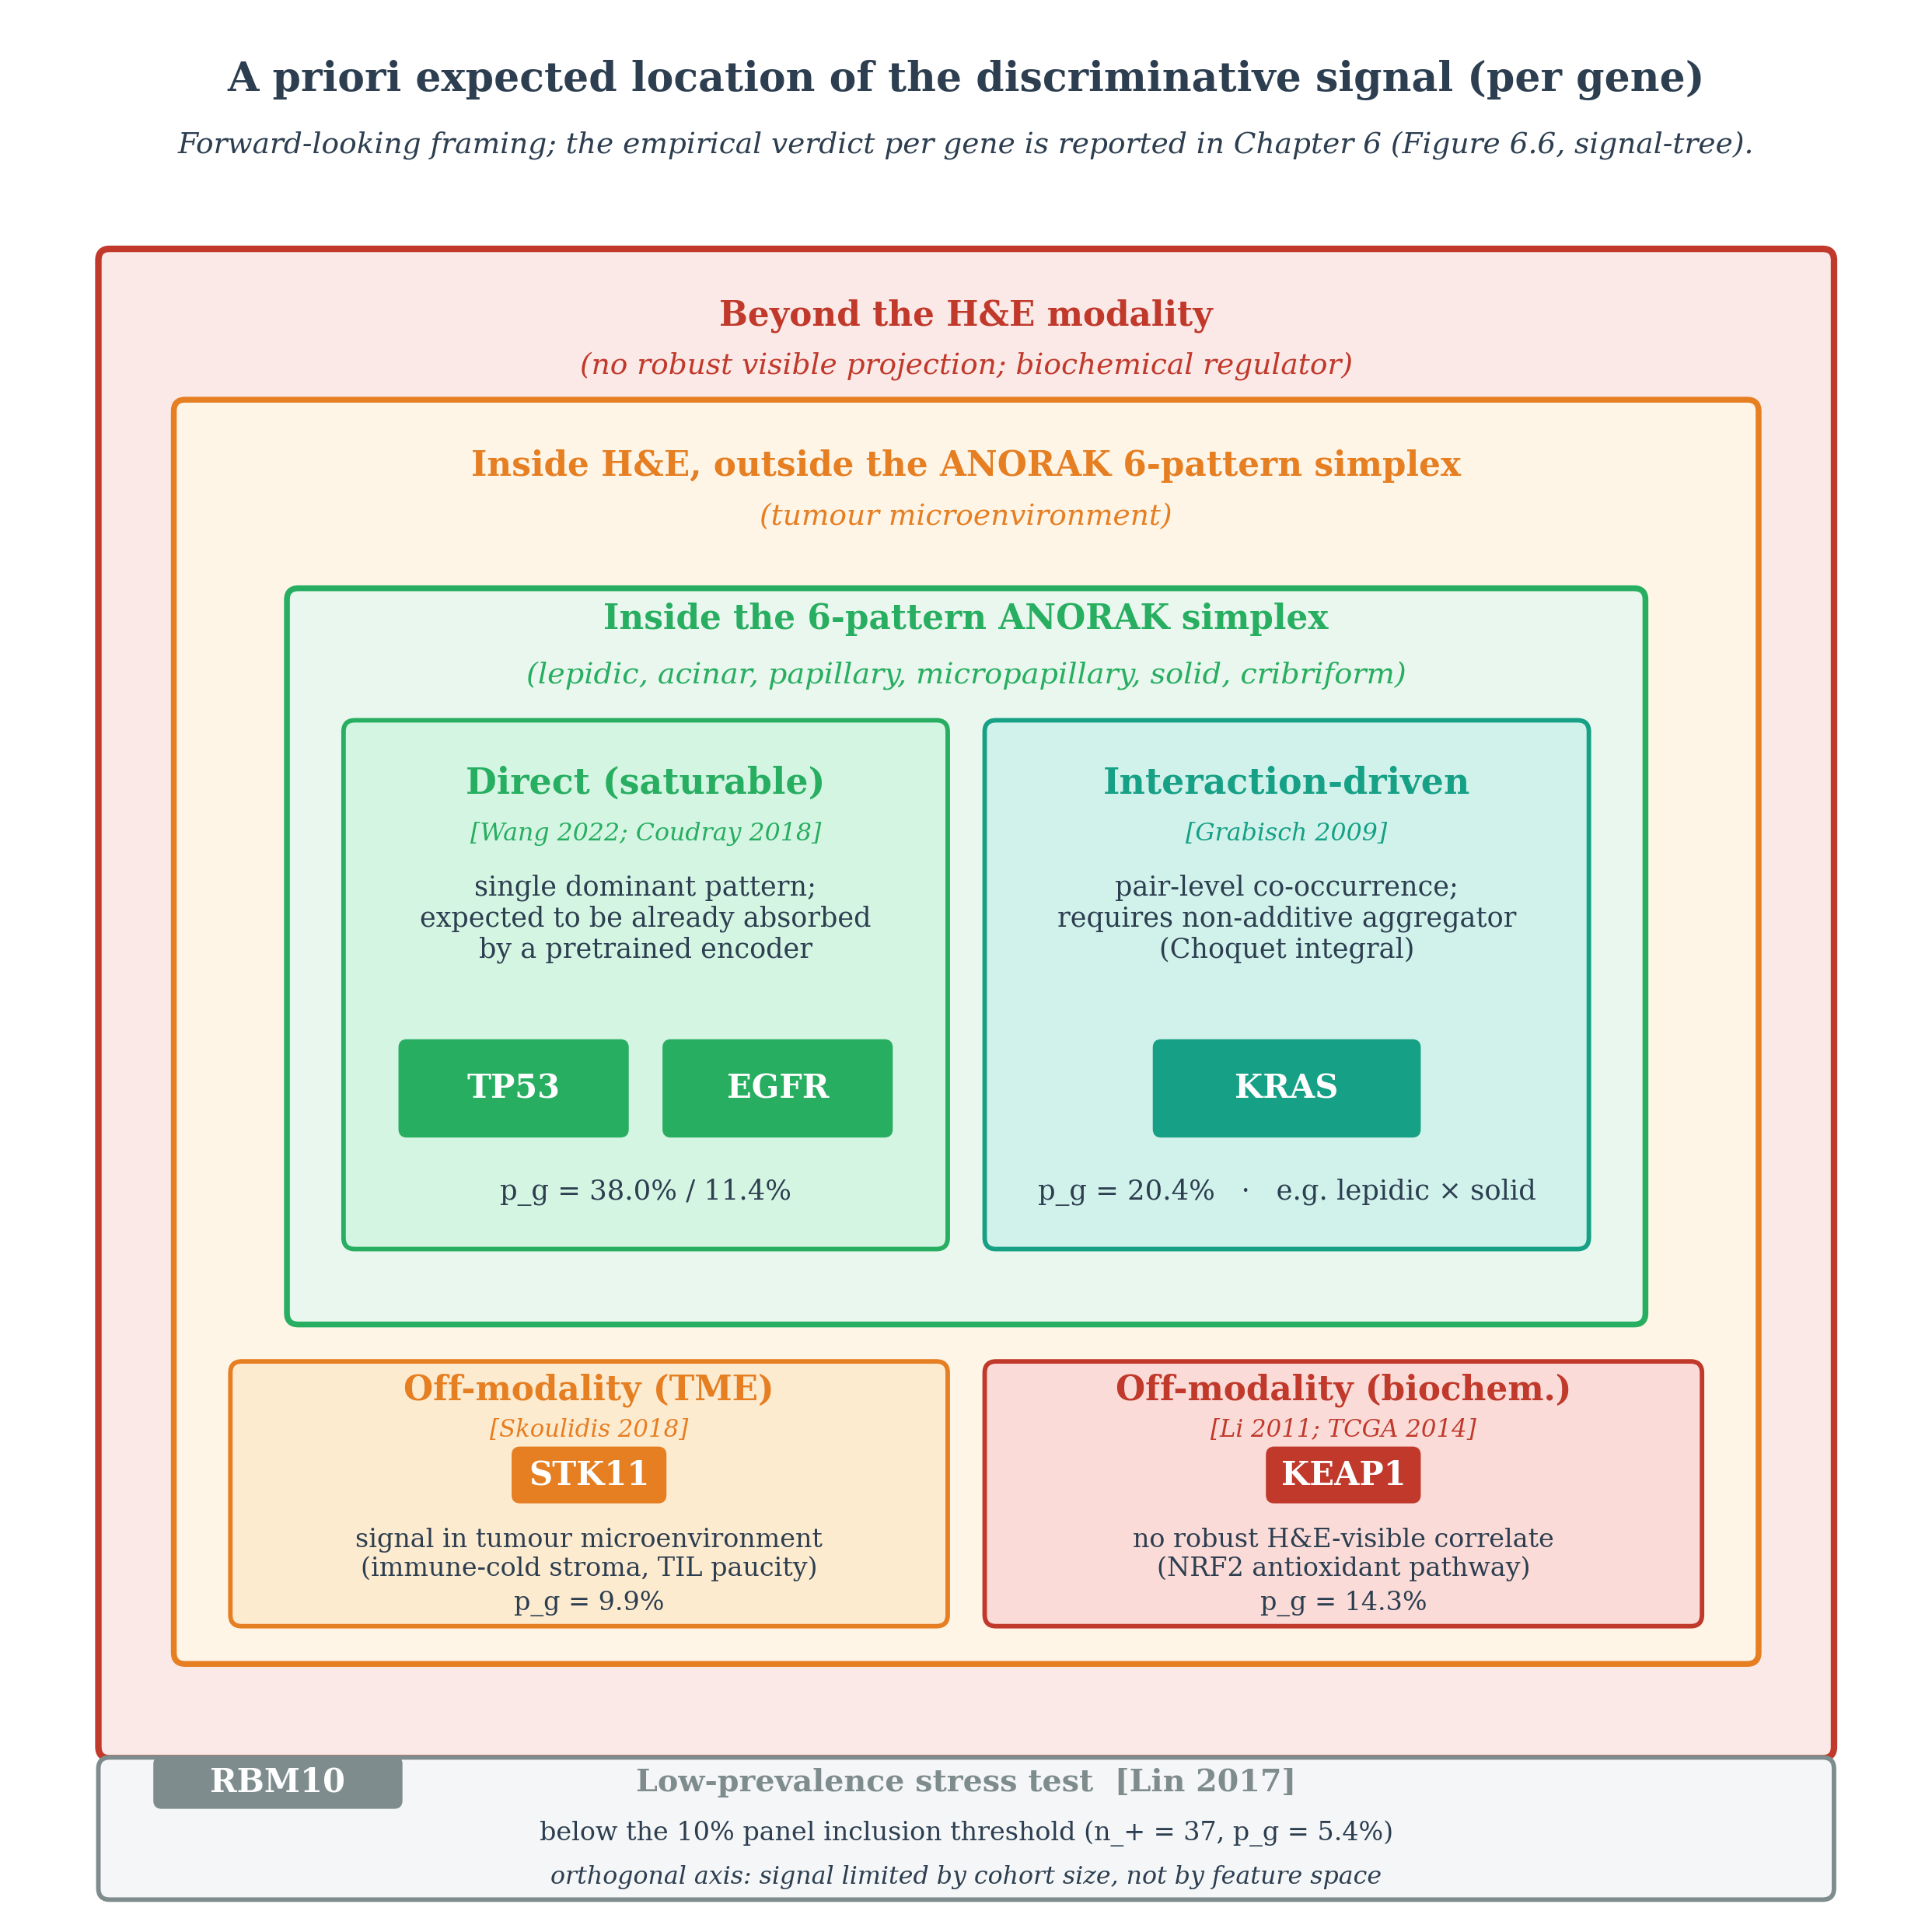
\includegraphics[width=\textwidth]{chapters/figures/luad_signal_scope.png}
    \caption[A priori signal-location scope diagram for the 6-gene
    panel]{%
        \emph{A priori} expected location of the discriminative
        signal for each of the six target genes, expressed as a scope
        diagram over the H\&E modality.
        The innermost (green) zone is the 6-pattern ANORAK simplex
        $\Delta^5$; it is split into a \textsc{Direct (saturable)}
        sub-zone (single dominant pattern, expected to be already
        absorbed by a pretrained encoder) hosting TP53 and EGFR, and
        an \textsc{Interaction-driven} sub-zone (pair-level
        co-occurrence, requiring a non-additive aggregator) hosting
        KRAS.
        The next ring out (orange) is still inside H\&E but outside
        the simplex---the tumour microenvironment, where STK11's
        \textsc{Off-modality (TME)} signal is expected to live.
        The outermost ring (red) lies beyond the H\&E modality
        altogether---an \textsc{Off-modality (biochemical)}
        regulator, where KEAP1's signal is expected.
        RBM10 is placed on a separate orthogonal axis (grey band)
        because its dominant constraint is cohort statistics
        ($n_+ = 37$) rather than feature-space coverage---the
        \textsc{Low-prevalence stress test} of the panel.
        This figure states the prior; the empirical verdict per gene
        is reported in Chapter~\ref{ch:evaluation}
        (Figure~\ref{fig:signal_tree}, the regime-tree synthesis), and
        the four failure mechanisms are visualised in
        Chapter~\ref{ch:discussion}
        (Figure~\ref{fig:genotype_phenotype_mismatch}).}
    \label{fig:luad_signal_scope}
\end{figure}


\subsection{Reading the Table: What Matters for Each Gene}
\label{sec:uc:gene_walkthrough}

For the reader who is new to cancer genomics, the following per-gene
walkthrough states the biology, the H\&E correlate, and the
\emph{a priori} expected discrimination mode of
Table~\ref{tab:gene_unified} for each of the six target genes.
The walkthrough is deliberately forward-looking: the empirical
verdict for each row of Table~\ref{tab:gene_unified} (which a priori
mode survives contact with the data, and through which mechanism)
is reported in Chapter~\ref{ch:evaluation} and synthesised into the
regime taxonomy of Figure~\ref{fig:signal_tree} (Ch.~\ref{ch:evaluation})
and Figure~\ref{fig:genotype_phenotype_mismatch}
(Ch.~\ref{ch:discussion}).

\textbf{\textit{TP53} --- The ``guardian of the genome.''}
When \textit{TP53} is mutated, the cell loses its primary mechanism
for detecting and repairing DNA damage.
The result is a tumour that grows aggressively and looks disorganised
under the microscope: large, irregular nuclei, frequent cell division,
and solid sheets of tumour cells.
The high-grade phenotype is visually distinctive in
H\&E~\cite{ahn2022tp53highgrade},
which is why Table~\ref{tab:gene_unified} assigns TP53 the
\textsc{Direct (saturable)} a priori mode---a strong single-pattern
correlate that a pretrained encoder is therefore likely to absorb on
its own.
No targeted drug exists for TP53; treatment relies on chemotherapy and,
when tumour mutation burden is high, immunotherapy.

\textbf{\textit{KRAS} --- The ``stuck switch.''}
The KRAS protein normally toggles between ``on'' and ``off'' states to
regulate cell growth; a mutation locks it in the ``on'' position,
driving continuous proliferation.
In the lung, this often manifests as the invasive mucinous variant
(IMA): tumour cells producing copious mucus, creating a distinctive
pale, gland-filled architecture~\cite{shim2015krasmucinous}.
Because IMA is a \emph{multi-pattern construct} (a mucinous acinar
phenotype with admixed lepidic and solid components rather than a
single dominant pattern), Table~\ref{tab:gene_unified} assigns KRAS
the \textsc{Interaction-driven} a priori mode: the discriminative
signal, if it exists, is expected to live in pairwise pattern
co-occurrence rather than in any single channel.
The G12C variant is now treatable with sotorasib and
adagrasib~\cite{skoulidis2021codebreak}; G12D (enriched in IMA) still
lacks an approved targeted agent.

\textbf{\textit{EGFR} --- The ``actionable target.''}
EGFR mutations are the most clinically important because effective
targeted drugs exist: patients receiving osimertinib (a
third-generation TKI) have substantially better
outcomes~\cite{soria2018flaura} than those given chemotherapy alone.
These tumours tend to grow in gentle, well-organised patterns
(lepidic and papillary) with relatively
normal-looking cells~\cite{yoshizawa2013egfrmorph}---a stark contrast
to the aggressive appearance of TP53-mutant tumours.
Like TP53, the literature signal is a single dominant phenotype;
Table~\ref{tab:gene_unified} therefore assigns EGFR the same
\textsc{Direct (saturable)} a priori mode.
The clinical motivation for slide-based prediction is acute in
settings where NGS is unavailable.

\textbf{\textit{STK11} --- The ``immune brake.''}
STK11 (also known as LKB1) normally helps recruit immune cells to
fight the tumour.
When STK11 is lost, the tumour becomes ``immune-cold''---there are few
lymphocytes (immune cells) in the surrounding
tissue~\cite{skoulidis2015krassubsets,skoulidis2018stk11pd1}.
This is visible in H\&E slides as an empty-looking stroma surrounding
the tumour.
Crucially, the signal lives in the \emph{surrounding tissue} rather
than in the tumour cells themselves, so it falls \emph{outside} the
six tumour-cell patterns of the ANORAK simplex.
Table~\ref{tab:gene_unified} therefore assigns STK11 the
\textsc{Off-modality (TME)} a priori mode: in H\&E but outside the
designed feature space.
Clinically, STK11 loss is a negative biomarker for immunotherapy
response.

\textbf{\textit{KEAP1} --- The ``metabolic shield.''}
KEAP1 mutations activate a cellular defence pathway (NRF2) that
protects the tumour from oxidative damage~\cite{tcga2014luad}.
Unlike TP53 or KRAS, KEAP1 loss does not produce a single dominant
morphological signature---although KEAP1 mutations are enriched in
papillary adenocarcinoma~\cite{li2011keap1papillary}, the overall
mutation--morphology relationship is biochemically indirect and less
well-characterised than for other driver genes.
Table~\ref{tab:gene_unified} therefore assigns KEAP1 the
\textsc{Off-modality (biochemical)} a priori mode: the regulatory
step is metabolic and may not project robustly into the H\&E modality
at all.

\textbf{\textit{RBM10} --- The ``low-prevalence floor.''}
RBM10 is an RNA-binding protein with no established microscopic
signature~\cite{tcga2014luad}; the predicted phenotype is RNA-splicing
dysregulation, a heterogeneous and indirect cellular consequence.
With $n_+ = 37$ mutated slides ($p_g = 5.4$\,\%), RBM10 is the
lowest-prevalence gene in the panel.
Table~\ref{tab:gene_unified} therefore assigns RBM10 the
\textsc{Low-prevalence stress test} a priori mode---the floor case
of the panel against which the discriminative power of any
condition is bounded by the cohort statistics rather than by the
algorithm.


\subsection{The Central Hypothesis}
\label{sec:uc:central_hypothesis}

The gene-specific morphological correlates summarised in
Table~\ref{tab:gene_unified} motivate the central hypothesis of this
thesis, stated formally in Chapter~\ref{ch:introduction}
(Section~\ref{sec:intro:hypothesis}) and reproduced here for
convenience:

\begin{quote}
\textbf{H:} \emph{Structured domain knowledge---specifically,
expert-defined histological growth patterns encoded through fuzzy set
theory---can be injected into a deep learning mutation prediction
pipeline to simultaneously
(a)~achieve competitive predictive performance under data scarcity
($<$700 public slides), and
(b)~render the resulting predictions \textbf{interpretable} through
a multi-level, clinically verifiable inspection framework---and,
through that framework, \textbf{explainable} via
knowledge-graph--grounded natural-language rationales---to a degree
that no end-to-end black-box approach offers.}
\end{quote}
The technical meaning of \emph{interpretable} and \emph{explainable}
in clause~(b) is the one established in
Section~\ref{sec:bg:xai:definitions}: the former is a structural
property of the model evaluated empirically in
Chapter~\ref{ch:evaluation}; the latter is a system capability whose
formal evaluation is reserved for future work
(Section~\ref{sec:disc:future}).

\textbf{Formalisation.}
With $\mathbf{x}_i \in \mathbb{R}^{512}$ the visual embedding and
$\mathbf{p}_i \in \Delta^5$ the fuzzy pattern membership vector
extracted by Artefact~1 from tile $i$ of slide~$s$, $\mathbf{H}$
predicts that an aggregator
$f: \{(\mathbf{x}_i, \mathbf{p}_i)\}_{i=1}^{N_s} \to [0,1]^6$
that consumes both channels strictly dominates an aggregator
$f': \{\mathbf{x}_i\}_{i=1}^{N_s} \to [0,1]^6$ that consumes only the
embedding, in the data-scarce regime $|\mathcal{S}| < 700$, and that
the resulting per-tile pattern channel makes the prediction auditable
in a way that the embedding-only baseline cannot.
The benchmark of Chapter~\ref{ch:evaluation} tests both clauses
(performance and interpretability) gene-by-gene; the
\emph{A priori mode} column of Table~\ref{tab:gene_unified} encodes
the prior per-gene expectation about \emph{how} (if at all) the
morphological signal projects into the 6-pattern simplex, against
which Chapter~\ref{ch:evaluation} compares the empirically observed
regime.


% ============================================================================
\section{Datasets}
\label{sec:uc:datasets}
% ============================================================================

This thesis uses two distinct datasets for two sequential tasks:
(1)~a curated expert-annotated dataset for training the histological
pattern classifier, and (2)~the TCGA-LUAD cohort for the downstream
mutation prediction task.
Table~\ref{tab:datasets_overview} provides a high-level summary, and
Table~\ref{tab:data_shape} gives the formal tensor-level shape that
each artefact actually consumes.

\begin{table}[ht!]
\centering
\caption{Overview of datasets used in this thesis.}
\label{tab:datasets_overview}
\begin{tabular}{p{3.5cm} p{2.5cm} p{2cm} p{2cm} p{3cm}}
\hline
\textbf{Dataset} & \textbf{Task} & \textbf{Samples} & \textbf{Classes} & \textbf{Labels} \\
\hline
Zenodo (Anorak) & Pattern classification & 637 tiles & 6 patterns & Expert pathologist \\
TCGA-LUAD & Mutation prediction & 687 WSIs & Binary per gene & WXS (MAF files) \\
\hline
\end{tabular}
\end{table}

\begin{table}[ht!]
\centering
\small
\caption{Tensor-level data shape consumed by each artefact.
``Sample'' means one independent unit of supervision; ``Bag'' means a
variable-size set of tiles drawn from the same WSI.
$N_s \in [\,5\,000, 80\,000\,]$ is the per-slide tile count.}
\label{tab:data_shape}
\resizebox{\textwidth}{!}{%
\begin{tabular}{l l l l l}
\hline
\textbf{Artefact} & \textbf{Sample type} & \textbf{Input shape} &
\textbf{Output shape} & \textbf{Cardinality} \\
\hline
A1 (FuzzyArcLoss V2)        & Tile     &
$\mathbb{R}^{4\times 224\times 224}$ (RGB+mask)         &
$\Delta^5$ (6-d simplex)        &
$|\mathcal{Z}| = 637$ tiles \\
A2 (PI-ABMIL)                & WSI bag  &
$\{(\mathbf{x}_i, \mathbf{p}_i)\}_{i=1}^{N_s}$, with
$\mathbf{x}_i \in \mathbb{R}^{512}$, $\mathbf{p}_i \in \Delta^5$ &
$[0,1]^6$ (per-gene)          &
$|\mathcal{S}| = 687$ WSIs / 668 patients \\
A3 (FC-MIL)                  & WSI bag  &
$\{\mathbf{p}_i\}_{i=1}^{N_s}$, $\mathbf{p}_i \in \Delta^5$
(plus shared $\mathbf{x}_i$ branch)                       &
$[0,1]^6$ (per-gene)          &
$|\mathcal{S}| = 687$ WSIs / 668 patients \\
\hline
\end{tabular}}
\end{table}


\subsection{Dataset 1: Zenodo Expert-Annotated Pattern Tiles}
\label{sec:uc:zenodo}

The histological pattern classifier was trained on an expert-annotated
dataset published on the Zenodo data repository, originally curated for
research on LUAD growth pattern recognition.
This dataset contains 637 image tiles extracted from H\&E-stained LUAD
whole-slide images, each annotated by a board-certified pathologist into
one of six growth pattern classes.

\textbf{Repository contents.}
The Zenodo repository (\texttt{10.5281/zenodo.10016027}) distributes
a single ZIP archive containing three components:
\begin{itemize}
    \item \textbf{H\&E tile images} --- 732 PNG/JPG files at
    $224 \times 224$ pixels, $20\times$ magnification.
    \item \textbf{Pixel-level annotation masks} --- 731 MATLAB
    binary files (\texttt{.mat}); one image lacks a mask.
    Each file contains an integer matrix of the same spatial
    dimensions as the corresponding tile, where every pixel is
    assigned a growth pattern class label (0--6).
    \item \textbf{Colour-coded annotation overlays} --- PNG images
    where the pathologist's annotation is rendered as a
    semi-transparent categorical colour map superimposed on the H\&E
    tile (Figure~\ref{fig:zenodo_overlays}).
    These overlays were used for visual verification during development
    but are \emph{not} part of the training pipeline.
\end{itemize}

\textbf{From 732 raw images to 637 usable tiles.}
Not all 732 images carry a valid growth pattern label.
Of the 731 tiles with annotation masks, 94 have a majority-vote label
of class~0 (``background/other''), meaning the tile contains no
diagnostically relevant tissue pattern; these are excluded.
The remaining \textbf{637 tiles across 6 classes} (including
cribriform, label~1) constitute the training dataset used
throughout this thesis (Table~\ref{tab:dataset_config_anorak}).

\textbf{From pixel masks to tile labels and overlays.}
The \texttt{.mat} masks encode the full spatial annotation provided by
the pathologist: each pixel of the $224 \times 224$ tile carries a
class integer indicating which growth pattern occupies that location.
The tile-level class label used for training is derived by
\emph{majority vote} over the non-zero pixels---i.e., the pattern that
covers the largest area of the tile determines the tile's label.
The colour-coded overlays are generated by
mapping each pixel's class integer to a fixed colour
(Table~\ref{tab:variant_types_patterns}) and alpha-blending the
result over the original H\&E image.
These overlays served two purposes in this thesis:
(i)~visual verification of model predictions during development
(comparing model-predicted pattern overlays against the expert
reference);
and (ii)~the binary tissue segmentation derived from the
\texttt{.mat} files is the source of the fourth channel of
Artefact~1's $4\times 224\times 224$ tile input (the dominant fix in
the pipeline audit; see Section~\ref{sec:uc:pipeline_fixes}).

\textbf{Spatial ground truth: a key difference from mutation labels.}
An important distinction between the two datasets used in this thesis
concerns the nature of their ground-truth labels.
The Zenodo--ANORAK \texttt{.mat} masks provide \emph{pixel-level
spatial ground truth}: a board-certified pathologist examined each
H\&E tile under the microscope and manually delineated where each
growth pattern is located, pixel by pixel.
The label and the image are in direct, one-to-one spatial
correspondence---if the mask says ``this pixel is acinar,'' the
pathologist visually confirmed acinar morphology at that exact location.
By contrast, the TCGA mutation labels derived from MAF files
(Section~\ref{sec:uc:tcga:maf}) are \emph{patient-level binary labels}
with no spatial information: the MAF says ``this patient has a TP53
missense mutation,'' but does not indicate where in the tissue the
phenotypic effect of that mutation is visible, because the mutation
was detected by bulk DNA sequencing of a macrodissected tissue fragment.
This distinction has a direct consequence for the two stages of the
pipeline:
\begin{itemize}
    \item \textbf{Stage~1 (Pattern classification):}
    The model is trained with spatially precise ground truth
    (\texttt{.mat} masks).
    Errors at this stage are classification errors---the model assigns
    the wrong pattern to a tile---but the ground truth itself is
    unambiguous.
    \item \textbf{Stage~3 (Mutation prediction):}
    The model is trained with patient-level labels that have no spatial
    correspondence to the image.
    Even a perfect model cannot be spatially verified against the MAF
    ground truth, because the MAF does not say \emph{where} in the
    slide the mutation manifests morphologically.
    This fundamental gap is discussed in
    Section~\ref{sec:disc:genotype_phenotype}.
\end{itemize}

\begin{table}[ht!]
\centering
\small
\caption{ANORAK annotation scheme: integer labels in the
\texttt{.mat} mask files and the overlay display colours used in
Figure~\ref{fig:zenodo_overlays}.
The \texttt{.mat} files encode pixel-level labels as integers (0--6);
the colour mapping is applied when rendering the semi-transparent
overlays onto the H\&E tiles.
Background (label~0) tiles are excluded.}
\label{tab:variant_types_patterns}
\begin{tabular}{c l l l}
\hline
\textbf{Label} & \textbf{Pattern} & \textbf{Overlay colour} & \textbf{Used?} \\
\hline
0 & Background / other    & Black (not rendered)  & Excluded \\
1 & Cribriform            & Cyan                  & Yes \\
2 & Micropapillary        & Green                 & Yes \\
3 & Solid                 & Dark red (maroon)     & Yes \\
4 & Papillary             & Yellow                & Yes \\
5 & Acinar                & Red                   & Yes \\
6 & Lepidic               & Blue                  & Yes \\
\hline
\end{tabular}
\end{table}

\textbf{Annotation protocol.}
Each tile was extracted at $20\times$ magnification with a size of
$224 \times 224$ pixels (roughly the field of view a pathologist sees
at medium power).
The pathologist assigned a pixel-level annotation mask
(\texttt{.mat} file) per tile, from which a single tile-level
label was derived by majority vote over the annotated pixels.
In addition to the annotation masks, binary tissue segmentation masks
were provided, delineating the neoplastic (cancerous) regions from
background (glass, pen marks, out-of-focus areas) and non-tumour tissue
(stroma, necrosis, inflammation).

\textbf{Class distribution.}
The dataset exhibits moderate class imbalance, as shown in
Table~\ref{tab:dataset_config_anorak}.
The micropapillary and cribriform classes are tied as the smallest
(55 training tiles each), while acinar is the most represented
(145 training tiles).

\begin{table}[ht!]
\centering
\small
\caption{Histological pattern distribution in the Zenodo ANORAK
dataset as used in this thesis.
Of 732 raw images in the repository, 731 have annotation masks;
after excluding 94 \emph{none}-class tiles (background/other),
637 are retained across the 6 ANORAK classes.
Training-set counts ($\approx$509 tiles) are estimated from the
stratified 80/20 split; full-dataset counts are exact.}
\label{tab:dataset_config_anorak}
\begin{tabular}{l r r r}
\hline
\textbf{Histological Pattern} &
\textbf{Training ($\approx$509)} &
\textbf{Full dataset (637)} &
\textbf{\%} \\
\hline
Acinar         & 145 & 181 & 28.4 \\
Papillary      & 100 & 125 & 19.6 \\
Solid          &  85 & 107 & 16.8 \\
Lepidic        &  69 &  86 & 13.5 \\
Micropapillary &  55 &  69 & 10.8 \\
Cribriform     &  55 &  69 & 10.8 \\
\hline
\textbf{Total} & \textbf{509} & \textbf{637} & \textbf{100.0} \\
\hline
\end{tabular}
\begin{flushleft}
\footnotesize
Split: 80/20 stratified by class (509 training, 128 test).
Micropapillary and cribriform are the minority classes with 55
training tiles each (10.8\%), motivating the adaptive fuzzy margin
of FuzzyArcLoss~V2.
Mean tiles per class: $\sim$106; range: 69--181 (acinar).
K-fold evaluation uses all 637 tiles with 5-fold
$\times$ 3-seed cross-validation (15 runs per method).
\end{flushleft}
\end{table}

This limited dataset size has two important consequences: first, it
constrains the complexity of the classification model (favouring
parameter-efficient architectures); second, it necessitates training
strategies that are robust to small-sample regimes, such as strong data
augmentation and angular margin losses that enforce well-separated
embeddings.

\textbf{4-Channel input.}
A key methodological decision, identified through systematic ablation
(Section~\ref{sec:uc:pipeline_fixes}), was to concatenate the binary
tissue segmentation mask as a fourth channel to the RGB input, producing
a $224 \times 224 \times 4$ tensor.
This spatial prior explicitly informs the model about the location of
diagnostically relevant tissue within each tile, eliminating the need to
learn tissue-versus-background discrimination from limited training data;
without this mask, classification performance drops by an estimated
15--20 percentage points across all loss functions
(Section~\ref{sec:uc:pipeline_fixes}).

\textbf{Data split.}
An 80/20 train/test split was used, stratified by class.
No validation set was held out; instead, model selection was performed
based on average precision (avgPR) on the test set, monitored every
epoch with early stopping patience.
For the final K-fold evaluation (5-fold $\times$ 3 seeds = 15 runs),
the entire dataset was used with stratified cross-validation.


\subsection{Dataset 2: TCGA-LUAD Whole-Slide Images and Mutation Data}
\label{sec:uc:tcga}

The Cancer Genome Atlas Lung Adenocarcinoma project (TCGA-LUAD) is a
publicly available multi-institutional genomic and histopathological
dataset curated by the National Cancer Institute (NCI) Genomic Data
Commons (GDC)~\cite{tcga2014luad}.
It is the largest public resource that provides \emph{both} digitised
histology slides and matched molecular profiling data for LUAD.

\subsubsection{Whole-Slide Images}

TCGA-LUAD provides formalin-fixed, paraffin-embedded (FFPE) diagnostic
whole-slide images in Aperio SVS format.
Each WSI was digitised at $20\times$ or $40\times$ magnification using
scanners at contributing institutions across the United States.
The slides are publicly accessible without controlled-access approval.

From the TCGA-LUAD project on the GDC---which has expanded since its
initial release---687 slides from 668 unique LUAD patients were
successfully downloaded and processed.
Of these 668 patients, 19 contributed more than one slide (e.g.\ both a
diagnostic DX and a tissue-sample BS section), yielding 687 slides in
total.
Patient-level stratification was applied throughout all cross-validation
experiments to prevent data leakage between slides from the same patient.

\textbf{Slide characteristics.}
Each WSI contains between 5,000 and 80,000 tissue-containing tiles at
$20\times$ magnification after background filtering (Otsu thresholding
on the saturation channel in HSV colour space).
The median slide contains approximately 25,000 tiles.
Tiles were extracted at $224 \times 224$ pixels without overlap, and
tiles with less than 50\% tissue content were discarded.


\subsubsection{Types of Somatic Mutations}
\label{sec:uc:tcga:variant_types}

Before describing the mutation data files, a brief primer on the types
of somatic mutations is essential for understanding how the binary
``mutated / wild-type'' labels used throughout this thesis are derived.
When a tumour acquires a change in its DNA, the functional consequence
depends on \emph{how} the protein-coding sequence is altered.
Table~\ref{tab:variant_types} summarises the variant classifications
relevant to this work, ordered by frequency in the TCGA-LUAD cohort.

\begin{table}[ht!]
\centering
\small
\caption{Somatic mutation variant classifications in the TCGA-LUAD
MAF file.
\emph{Non-silent} variants (top group) alter the protein product and
are retained as positive mutation labels.
\emph{Silent} and non-coding variants (bottom group) are excluded.
Counts are from the first 50,000 records of the GDC Masked Somatic
Mutation file (LUAD only).}
\label{tab:variant_types}
\begin{tabular}{l l l}
\hline
\textbf{Variant Classification} & \textbf{Effect on protein} & \textbf{Retained?} \\
\hline
\texttt{Missense\_Mutation}  & Single amino acid substitution         & Yes \\
\texttt{Nonsense\_Mutation}  & Premature stop codon (truncated protein) & Yes \\
\texttt{Frame\_Shift\_Del}   & Deletion disrupting the reading frame   & Yes \\
\texttt{Splice\_Site}        & Alters mRNA splicing at exon--intron boundary & Yes \\
\texttt{Frame\_Shift\_Ins}   & Insertion disrupting the reading frame  & Yes \\
\texttt{In\_Frame\_Del}      & Deletion preserving the reading frame   & Yes \\
\texttt{In\_Frame\_Ins}      & Insertion preserving the reading frame  & Yes \\
\hline
\texttt{Silent}              & Synonymous; DNA changes but protein unchanged & No \\
\texttt{Intron}              & Within a non-coding intron region       & No \\
\texttt{RNA}                 & Non-coding RNA region                   & No \\
\texttt{Splice\_Region}      & Near (but not at) a splice site         & No \\
\texttt{3'UTR / 5'UTR}       & Untranslated regions flanking the gene  & No \\
\hline
\end{tabular}
\end{table}

A gene is labelled ``mutated'' for a patient if \emph{at least one}
non-silent variant from the top group of Table~\ref{tab:variant_types}
is detected in that gene.
In the TCGA-LUAD cohort, \texttt{Missense\_Mutation} accounts for
approximately 65\% of all recorded somatic variants, followed by
\texttt{Silent} (22\%, excluded), \texttt{Nonsense\_Mutation} (5\%),
and frameshift events (3\%).
The dominance of missense mutations means that most ``mutated'' labels
reflect a single amino acid change rather than a complete loss of the
protein---an important consideration when interpreting morphological
correlates, because the phenotypic effect of a missense mutation
varies from negligible to severe depending on its location in the
protein structure.


\subsubsection{Mutation Annotation Format (MAF) Files}
\label{sec:uc:tcga:maf}

The mutation labels used throughout this thesis are derived from the
Genomic Data Commons (GDC) \emph{Masked Somatic Mutation} files in
MAF format~\cite{gdc2024maf}.

\textbf{What is a MAF file?}
A MAF file is a plain-text, tab-delimited table (not an image or
binary format) where each row represents one somatic mutation detected
in one patient.
The TCGA-LUAD MAF file contains 140 columns and approximately 230\,MB
of text.
The columns most relevant to this thesis are:
\begin{description}[leftmargin=2.5cm, style=nextline]
    \item[\texttt{Hugo\_Symbol}] The gene name (e.g., \texttt{TP53},
    \texttt{KRAS}).
    \item[\texttt{Chromosome}, \texttt{Start/End\_Position}]
    Genomic coordinates of the mutation on the GRCh38 reference genome.
    \item[\texttt{Variant\_Classification}] The functional consequence
    of the mutation (Table~\ref{tab:variant_types}).
    \item[\texttt{Tumor\_Sample\_Barcode}] The TCGA patient identifier
    (e.g., \texttt{TCGA-69-7979-01A-11D-2184-08}), from which the
    first 12 characters (\texttt{TCGA-69-7979}) serve as the
    patient-level key that links this mutation record to the
    corresponding whole-slide image(s).
    \item[\texttt{Reference/Tumor\_Seq\_Allele}] The original (normal)
    and mutated DNA bases.
\end{description}

\textbf{Linking MAF data to histology images.}
It is important to emphasise that MAF files contain \emph{no image
data whatsoever}---they are purely genomic records.
The connection between a mutation and its histological slide is
established through the shared TCGA patient barcode: the first 12
characters of \texttt{Tumor\_Sample\_Barcode} in the MAF file
(e.g., \texttt{TCGA-55-7815}) match the barcode embedded in the
whole-slide image filename
(e.g., \texttt{TCGA-55-7815-01A-01-TS1.svs}).
This barcode-based join produces the final analysis matrix: for each
of the 687 slides, a binary label vector indicating which of the six
target genes carry at least one non-silent somatic mutation.

\textbf{Bioinformatics pipeline (upstream of this thesis).}
The MAF file is the output of a bioinformatics pipeline that the reader
does not need to reproduce but should understand at a high level:
\begin{enumerate}
    \item \textbf{Whole-exome sequencing (WXS):} DNA from each patient's
    tumour and matched normal blood sample was sequenced, covering all
    protein-coding regions of the genome ($\sim$2\% of total DNA).
    \item \textbf{Variant calling (MuTect2):} Sequencing reads from
    the tumour were compared against the normal sample to identify
    positions where the tumour DNA differs from the patient's own
    germline---these differences are \emph{somatic mutations},
    acquired by the tumour during its development.
    \item \textbf{Masking (quality filtering):} The GDC applies
    conservative filters to remove likely false positives: variants
    found in the general population database (dbSNP) without a COSMIC
    match (i.e., not previously seen in cancer), variants flagged by a
    Panel of Normals (recurrent sequencing artefacts), and variants in
    non-coding regions.
    The resulting ``masked'' MAF file contains only high-confidence
    somatic mutations and is publicly available without
    controlled-access restrictions.
\end{enumerate}


\subsubsection{Target Genes and Mutation Prevalence}
\label{sec:uc:tcga:genes}

Six genes were selected for mutation prediction based on their clinical
relevance and mutation prevalence in the LUAD cohort.
Following the inclusion criterion established by
Coudray~et~al.~\cite{coudray2018classification}---a minimum mutation
prevalence of 10\% to ensure sufficient positive cases for model
training---five genes met this threshold.
\textit{RBM10} (5.4\,\% prevalence) was included as the
\textsc{Low-prevalence stress test} row of
Table~\ref{tab:gene_unified}---the floor case below the 10\,\%
inclusion threshold---to characterise per-gene behaviour at the
lower end of the panel's prevalence range.

Table~\ref{tab:mutation_prevalence} reports the mutation counts and
prevalence for the 687 LUAD slides used in the primary analysis.
Each of the 687 slides carries an independent binary label
(``mutated'' or ``wild-type'') for \emph{each} of the six genes---a
single slide can be simultaneously mutated for one gene and wild-type
for another.
Therefore, in each row of the table, the ``Mutated'' and ``Wild-type''
columns sum to 687 (the total number of slides), not to the number of
distinct mutations.

\begin{table}[ht!]
\centering
\caption{Mutation prevalence in the TCGA-LUAD cohort
(687 slides from 668 patients with available WSIs).
Genes are ordered by decreasing prevalence.
The 10\% inclusion threshold of
Coudray~et~al.~\cite{coudray2018classification} is indicated.}
\label{tab:mutation_prevalence}
\begin{tabular}{l r r r l}
\hline
\textbf{Gene} & \textbf{Mutated} & \textbf{Wild-type} &
\textbf{Prevalence (\%)} & \textbf{$\geq$ 10\% threshold} \\
\hline
\textit{TP53}   & 261 & 426 & 38.0 & \checkmark \\
\textit{KRAS}   & 140 & 547 & 20.4 & \checkmark \\
\textit{KEAP1}  &  98 & 589 & 14.3 & \checkmark \\
\textit{EGFR}   &  78 & 609 & 11.4 & \checkmark \\
\textit{STK11}  &  68 & 619 &  9.9 & $\approx$\checkmark$^{\dagger}$ \\
\textit{RBM10}  &  37 & 650 &  5.4 & $\times$ \\
\hline
\end{tabular}
\begin{flushleft}
\footnotesize
$^{\dagger}$\textit{STK11} prevalence (9.9\%) falls marginally below the
10\% threshold.
It is retained because its known association with the immune
microenvironment (cold tumour phenotype visible in H\&E) makes it
a clinically relevant test case, and the absolute number of positive
cases (68) is sufficient for 5-fold cross-validation with $\geq$13
positive cases per fold on average.
\end{flushleft}
\end{table}


\subsection{Histopathology Slide Preparation and Digitalisation}
\label{sec:uc:he_acquisition}

Whole-slide images used for model training and quantitative evaluation in
this thesis are derived exclusively from publicly available research
datasets: the Zenodo ANORAK dataset for patch-level morphological
supervision and TCGA-LUAD for case-level molecular association
(Section~\ref{sec:uc:datasets}).
No proprietary clinical whole-slide images obtained at external hospitals
were used for algorithm training, testing, or quantitative analysis.

Nevertheless, an understanding of the standard clinical histopathology
workflow is essential to correctly interpret the sources of visual
variability present in real-world H\&E images.
Clinical observation and expert discussion at SOLCA (Sociedad de Lucha
Contra el Cáncer, Ecuador) were used to contextualise the image
formation process underlying digital histopathology.
In routine diagnostic practice, tissue specimens are fixed in formalin
(a preservative), embedded in paraffin wax (to make them firm enough to
cut), sectioned into thin slices, stained with H\&E, and subsequently
digitised using whole-slide scanners.

Figure~\ref{fig:he_pipeline_solca} schematically illustrates this
end-to-end acquisition pipeline, highlighting common sources of visual
variability---staining intensity, scanner optics, section thickness, and
preprocessing---that motivate the use of robust, noise-aware learning
objectives in this thesis.

\begin{figure}[ht!]
  \centering
  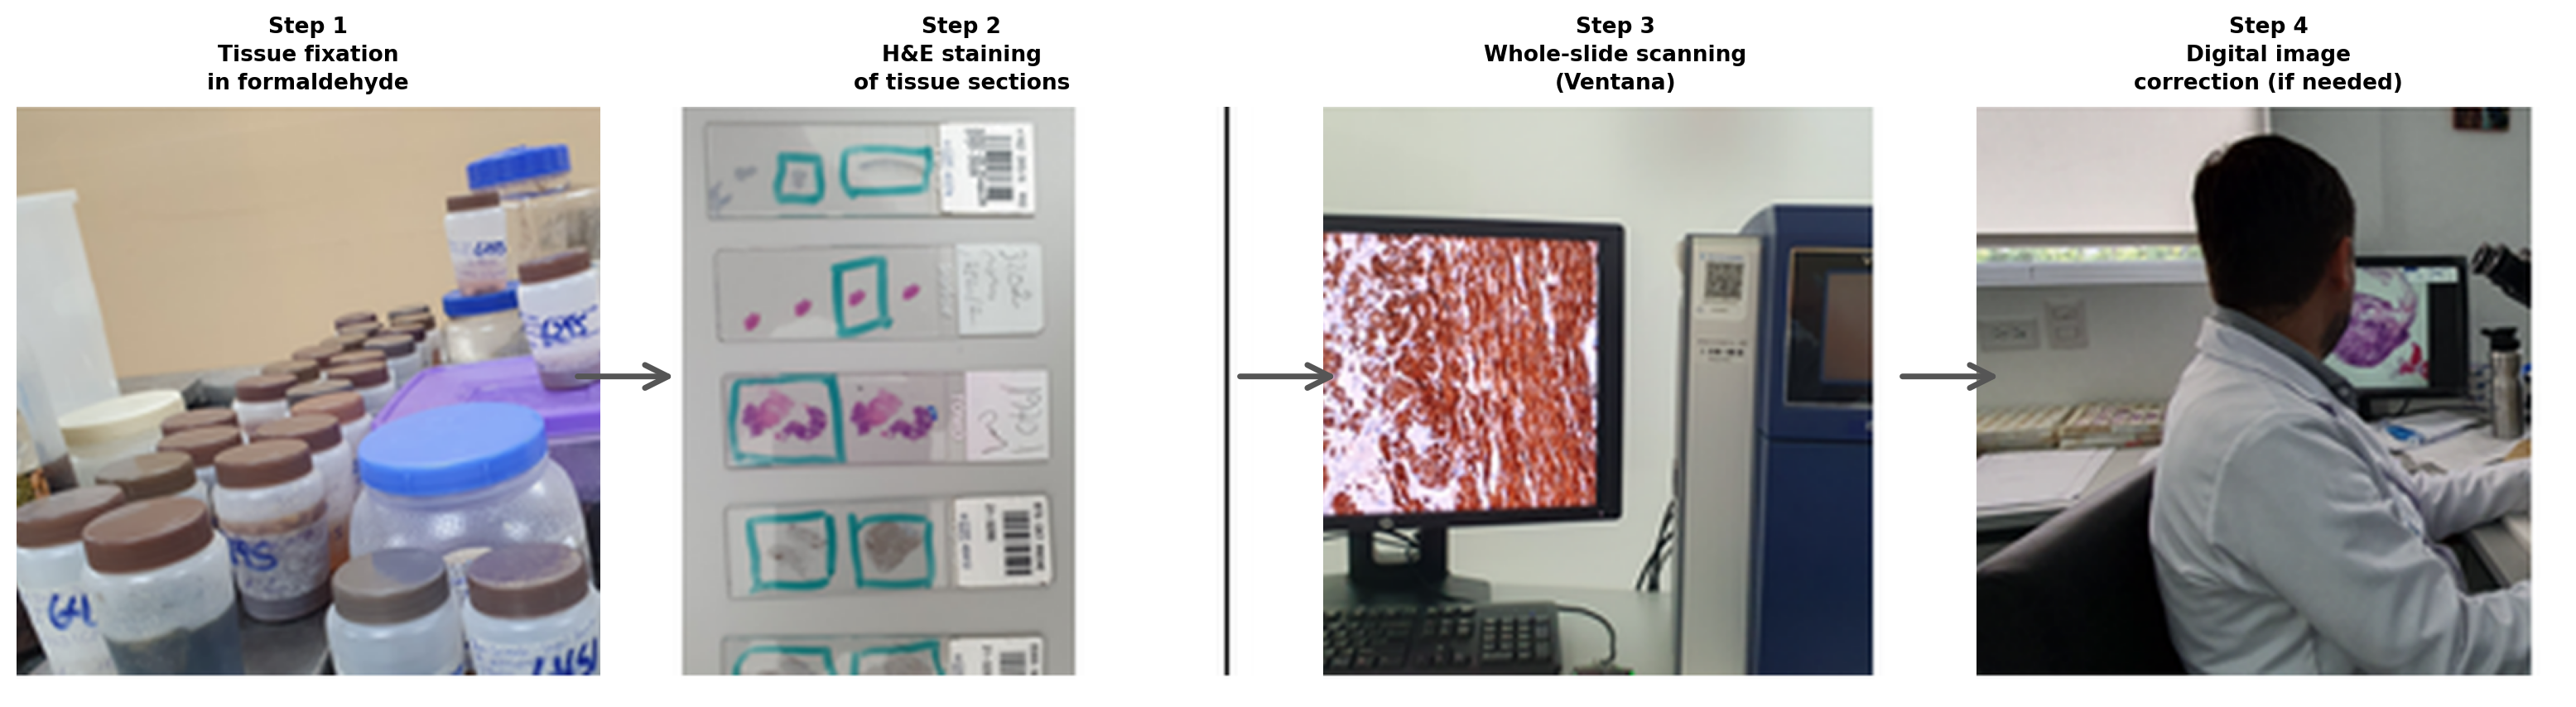
\includegraphics[width=\textwidth]{chapters/figures/he_workflow_solca.png}
  \caption[Standard H\&E histopathology acquisition pipeline]{%
      Standard clinical workflow for digital H\&E histopathology.
      Tissue fixation and paraffin embedding are followed by sectioning,
      haematoxylin and eosin staining, whole-slide scanning, and optional
      image correction (stain normalisation, background removal).
      Key sources of inter-slide variability are indicated at each stage:
      formalin concentration and fixation time affect nuclear staining
      intensity; section thickness affects tile contrast; scanner optics
      and gain settings affect colour temperature.
      These sources of variability justify the use of FuzzyArcLoss~V2's
      adaptive margins, which reduce the penalty for tiles whose
      morphological ambiguity arises from acquisition variation rather
      than true class overlap.
      Images and workflow are representative of clinical practice as
      observed at SOLCA Ecuador, used here for didactic and contextual
      purposes only.}
  \label{fig:he_pipeline_solca}
\end{figure}

\textbf{Role of SOLCA in this thesis.}
SOLCA contributed domain expertise through clinical consultation and
review of representative H\&E slide examples, informing the
morphological descriptions in Section~\ref{sec:uc:luad_histology} and
the clinical plausibility assessment of the attention maps
(Section~\ref{sec:eval:interpretability}).
No patient data from SOLCA enters the computational pipeline.


\subsection{TCGA-LUAD Mutation Calls and Case-Level Linking}
\label{subsec:tcga_mutations_linking}

Genetic alteration labels (TP53, EGFR, KRAS, STK11, KEAP1, RBM10) were
derived from somatic mutation calls provided by the TCGA-LUAD project
via the NCI Genomic Data Commons (GDC)~\cite{gdc2024maf}.
Mutation data were obtained in Masked Somatic Mutation MAF format, which
aggregates high-confidence somatic variants per tumour sample.

To associate genomic mutation data with histopathology images, all
records were linked at the patient level using the TCGA submitter barcode
convention.
Specifically, the first 12 characters of the TCGA barcode
(e.g., \texttt{TCGA-55-7815}) uniquely identify a patient and are shared
across molecular and imaging modalities:

\begin{equation}
\label{eq:barcode_linking}
\texttt{case\_barcode} = \texttt{substr(Tumor\_Sample\_Barcode,\,1,\,12)}.
\end{equation}

For WSIs, the same identifier is available as
\texttt{cases.submitter\_id} in the GDC API or as the prefix of extended
slide identifiers (e.g.,
\texttt{TCGA-55-7815-01A-01-TS1.xxx})~\cite{gdc2024maf}.
A deterministic join was performed to associate each WSI with the
corresponding case-level mutation status.

Three edge cases required explicit handling:
\begin{enumerate}
    \item \textbf{Multi-slide patients:} 19 patients contributed more
    than one slide (DX + BS sections). All slides from a patient were
    assigned to the same cross-validation fold to prevent data leakage.

    \item \textbf{Missing MAF entries:} slides with no matching MAF
    record were excluded from the analysis (all 687 slides in the
    final cohort have a valid mutation label for all 6 genes).

    \item \textbf{Ambiguous variants:} only non-silent somatic mutations
    (Missense, Nonsense, Frame-shift, Splice-site, In-frame indels) were
    counted as ``mutated''; synonymous variants were excluded.
\end{enumerate}

This barcode-based linkage is the standard mechanism by which TCGA
enables integration of molecular and histopathological data across
repositories and was verified to produce a $687 \times 6$ mutation
label matrix with no missing values
(Section~\ref{sec:impl:data_completeness}).


\subsubsection{The LUAD-Only Decision}
\label{sec:uc:tcga:luad_only}

The benchmark is restricted to LUAD slides because four of the six
target genes (\textit{EGFR}, \textit{KRAS}, \textit{STK11},
\textit{RBM10}) are almost exclusively LUAD-associated, with near-zero
prevalence in lung squamous cell carcinoma (LUSC).
Pooling LUAD with LUSC would let LUSC slides act as morphologically
distinct ``easy negatives'' for these genes: the classifier could
separate LUSC from LUAD-mutant by overall histology rather than by
mutation-associated features \emph{within} adenocarcinoma, inflating
AUROC without testing the within-LUAD discrimination that is
clinically relevant.
The remaining two genes (\textit{TP53}, \textit{KEAP1}) are mutated
in both subtypes, but mixing cohorts to support them would compromise
the four LUAD-specific genes that constitute the more challenging
prediction task.

The LUAD-only cohort ($N = 687$ slides, 668 patients) therefore
represents a harder but more clinically relevant benchmark.
All results reported in this thesis are based on the LUAD-only
analysis.


\subsection{Potential External Validation Cohorts}
\label{sec:uc:external}

Three additional public datasets were identified for potential external
validation in future work.
Table~\ref{tab:external_cohorts} summarises their key characteristics.

\begin{itemize}
    \item \textbf{CPTAC-3 LUAD} ($\sim$111 patients): The Clinical
    Proteomic Tumor Analysis Consortium Phase~3. Multi-institutional
    cohort from the United States with whole-exome sequencing and SVS
    slides available through the GDC.

    \item \textbf{APOLLO-LUAD} ($\sim$87 patients): The Applied
    Proteogenomics OrganizationaL Learning and Outcomes consortium.
    A Department of Defence/Veterans Affairs network with whole-genome
    sequencing and proteogenomic characterisation.

    \item \textbf{CDDP\_EAGLE-1} ($\sim$31 LUAD patients): An Italian
    cohort from the Environment And Genetics in Lung cancer Etiology
    study, collected from hospitals in Lombardy (2002--2005).
    Provides geographic and ethnic diversity not present in TCGA.
\end{itemize}

\begin{table}[ht!]
\centering
\caption{External LUAD cohorts with public WSIs and mutation data
identified for future validation.}
\label{tab:external_cohorts}
\begin{tabular}{l r l l l}
\hline
\textbf{Cohort} & \textbf{$N$ (approx.)} & \textbf{Sequencing} &
\textbf{Origin} & \textbf{Source} \\
\hline
CPTAC-3 LUAD    & 111 & WXS      & Multi-site, USA    & GDC \\
APOLLO-LUAD     &  87 & WGS      & DoD/VA, USA        & GDC/TCIA \\
CDDP\_EAGLE-1   &  31 & WGS/WXS  & Lombardy, Italy    & GDC \\
\hline
\textbf{Total external} & \textbf{229} & & & \\
\hline
\end{tabular}
\end{table}

Together, these cohorts add approximately 229 patients to the 668 used
in this thesis, bringing the total publicly available LUAD data with
both WSIs and mutation annotations to approximately \textbf{897 cases}.
No additional public sources with both modalities were identified after
exhaustive search.

\paragraph{Why external cohorts are not incorporated in this thesis.}
Despite their availability, the three external cohorts were not
incorporated into the benchmark experiments for three reasons:
pooling all public cohorts yields $\sim$897 slides---still two orders of
magnitude below proprietary state-of-the-art systems such as CHIEF
(60,530 slides~\cite{wang2024chief}) and GigaPath
($\sim$1.3 billion tiles~\cite{xu2024gigapath}), so the scale gain does
not change the data scarcity constraint that motivates the methodology
of this thesis;
combining cohorts from different scanners and staining protocols
introduces batch effects requiring normalisation beyond the scope of
this work;
and the variant-calling pipelines of CPTAC-3, APOLLO, and EAGLE differ
from the TCGA MAF format, requiring bioinformatic harmonisation that
falls outside the histopathology focus of this thesis.


% ============================================================================
\section{The Data Scarcity Challenge}
\label{sec:uc:data_scarcity}
% ============================================================================

A defining characteristic of this use case---and a central motivation
for the fuzzy-logic-based methodology---is the severe limitation in
available data relative to the state of the art.

\subsection{Scale Comparison with the Literature}
\label{sec:uc:data_scarcity:comparison}

Table~\ref{tab:data_scale} compares the data available for this thesis
with the datasets used by leading studies.
The gap is on the order of $\Delta\log_{10}(N) \approx 2$:
from $\sim 700$ public WSIs available to this thesis to
$\sim 6 \times 10^4$ proprietary slides
($\sim 1.3 \times 10^9$ tiles) used by current foundation models---a
two-order-of-magnitude difference that is \emph{not closable} through
additional data collection within the scope of a doctoral thesis.
This gap is the \textbf{operational definition of ``data scarcity''}
used in the rest of this thesis, and the corresponding methodological
response is the central hypothesis $\mathbf{H}$ stated in
Section~\ref{sec:uc:central_hypothesis}.

\begin{table}[ht!]
\centering
\caption{Data scale comparison. Proprietary datasets are inaccessible to
external researchers.}
\label{tab:data_scale}
\begin{tabular}{l r l l}
\hline
\textbf{Study / Dataset} & \textbf{Patients} & \textbf{Data access} &
\textbf{Source} \\
\hline
\textbf{This thesis} & \textbf{668} & \textbf{Public} &
\textbf{TCGA-LUAD} \\
\hline
Coudray et al.~\cite{coudray2018classification} & 382 & Public & TCGA-LUAD \\
Saldanha et al.~\cite{saldanha2023npj} & 676 & Public & TCGA + CPTAC \\
Logan et al.~\cite{logan2022medrxiv} & 747 & Mixed & DHMC + CPTAC \\
GAMIL~\cite{gamil2025diagpath} & 2,221 & Proprietary & Chinese hospitals \\
Zhao / DeepGEM~\cite{zhao2025deepgem} & 3,637 & Proprietary & 16 Chinese hospitals \\
Campanella / EAGLE~\cite{campanella2025eagle} & 8,461 & Proprietary & Microsoft + hospitals \\
Wang / CHIEF~\cite{wang2024chief} & 60,530 & Proprietary & Hospital networks \\
Xu / GigaPath~\cite{xu2024gigapath} & $\sim$1.3B tiles & Proprietary & Providence Health \\
\hline
\end{tabular}
\end{table}


\subsection{Implications: Why This Use Case Demands the Methodology of Chapter~\ref{ch:methodology}}
\label{sec:uc:data_scarcity:implications}

The data scarcity quantified above is not just a difficulty---it is
the \emph{driver} of three concrete design constraints, each
addressed by one of the artefacts of
Section~\ref{sec:uc:artifact_vision}.

\textbf{(i)~Parameter efficiency at the tile level.}
With approximately $637/6 \approx 106$ tiles per class in the ANORAK
training set, the pattern classifier cannot afford the parameter
budget of standard sub-centre or prototype-rich variants;
this constraint motivates the single-prototype-per-class design of
\textbf{FuzzyArcLoss V2} ($6 \times 512 = 3{,}072$ prototype
parameters) over heavier alternatives such as V3 SubCentres
(12{,}288 parameters at four sub-centres per class).

\textbf{(ii)~Structured priors at the slide level.}
With only $\sim 137$ slides per held-out fold
($687 / 5 \approx 137$) under 5-fold patient-stratified
cross-validation, an embedding-only aggregator must rediscover all
morphology--genotype associations from data;
the explicit injection of fuzzy pattern probabilities
$\mathbf{p}_i$ as a separate channel encodes the existing medical
knowledge so that the model does not have to rediscover, e.g.~that
solid morphology is enriched in \textit{TP53}-mutant tumours.
This is the design rationale for \textbf{Pattern-Informed ABMIL} and
\textbf{Fuzzy Choquet MIL}.

\textbf{(iii)~Variance-aware evaluation.}
With $\sim 137$ slides per held-out fold, single-split AUROC estimates are
high-variance ($\sigma_{\mathrm{AUROC}} \approx 0.05$--$0.10$ in
practice).
Reliable comparison therefore requires stratified $K$-fold
cross-validation with paired statistical tests and effect-size
reporting rather than headline AUROC differences---the evaluation
protocol adopted in Chapter~\ref{ch:methodology}.


% ============================================================================
\section{Research Questions: Use-Case-Specific Mapping}
\label{sec:uc:clinical_questions}
% ============================================================================

Chapter~\ref{ch:introduction} (Section~\ref{sec:intro:rq}) formulated
seven research questions (RQ1--RQ7) that operationalise the central
hypothesis $\mathbf{H}$ at the abstract methodological level.
This section does \emph{not} restate them; instead it makes the
mapping explicit between each RQ, the artefact that addresses it under
the LUAD use case, the evaluation method employed in
Chapter~\ref{ch:evaluation}, and the success criterion against which
the verdict is rendered.
The reader is referred to Section~\ref{sec:intro:rq} for the canonical
RQ wording (which decomposes RQ2 into RQ2(i) and RQ2(ii), and which
treats the DeepSearch outputs of RQ7 as \emph{candidate} relations
pending formal expert validation).

\begin{table}[ht!]
\centering
\small
\caption{Mapping of research questions to artefacts and evaluation
methods.}
\label{tab:rq_mapping}
\begin{tabular}{c p{3.8cm} p{3.5cm} p{3.5cm}}
\hline
\textbf{RQ} & \textbf{Artefact} & \textbf{Evaluation method} &
\textbf{Success criterion} \\
\hline
RQ1 & FuzzyArcLoss V2 & 5-fold $\times$ 3-seed macro-F1; paired
$t$-test vs baselines & V2 $\geq$ ArcFace mean F1; $p < 0.05$ vs
$\geq$1 baseline \\
RQ2(i) & Pattern-Informed ABMIL & 5-fold AUROC on 6 genes; comparison vs
ABMIL-emb (B2) & PI-ABMIL $\geq$ B2 mean AUROC on $\geq$1 gene \\
RQ2(ii) & Per-gene regime analysis & Three-regime taxonomy with
five named mechanisms: \emph{Regime A} (encoder saturation;
direct/saturable signal), \emph{Regime B} (out-of-ontology, three
sub-mechanisms: label-space mismatch, no morphological projection,
collapse-to-prior), and \emph{Regime C} (cross-term in label space) &
Each gene assigned to one regime with empirical evidence
(per-slide ablation, encoder swap, head replacement) \\
RQ3 & Fuzzy Choquet MIL & 5-fold AUROC per gene; Shapley
interaction analysis & Interpretable pairwise Shapley interactions;
FC-MIL leads on $\geq$1 gene where Regime~C (cross-term) applies \\
RQ4 & Six-level interpretability + fuzzy linguistic labels &
Qualitative: attention + pattern overlay + SHAP + Choquet Shapley +
ablation + fuzzy labels; LLM-prompt anti-hallucination check &
Six layers instrumented end-to-end; LLM intensity terms always drawn
from the deterministic fuzzy-label vocabulary \\
RQ5 & All artefacts combined & Performance gap analysis vs literature at
matched $N$ & Competitive with Saldanha (2023) and Logan (2022) \\
RQ6 & Ontology KG layer (LCHAI v2.0) &
  System demonstration: case graph rendering; provenance tags &
  Case-specific KG with typed entities and provenance demonstrated \\
RQ7 & DeepSearch pipeline (LCHAI v2.0) &
  Batch run: count candidate relations with provenance pointers and
  type-constraint validation &
  $\geq$1 candidate relation with PMID + NCIt/MONDO type check
  (formal expert validation deferred to future work) \\
\hline
\end{tabular}
\end{table}


% ============================================================================
\section{Systematic Pipeline Audit: Headline}
\label{sec:uc:pipeline_fixes}
% ============================================================================

Before any of the methodology of Chapter~\ref{ch:methodology} was
applied to the LUAD use case, a systematic audit of the pattern
classification training pipeline identified twenty implementation
issues---ten methodologically significant and ten low-impact code
fixes---whose correction raised macro-F1 uniformly by approximately
\textbf{18 percentage points (from 71--76\,\% to 89--95\,\% across all
18 loss-function variants)} on single-run evaluation.
The crucial property of this audit is \emph{uniformity}: every fix
affected all 18 losses equally, so the corrections establish a
\textbf{correct and fair experimental baseline} rather than
preferentially advantaging any one method.
The full list of fixes (4-channel input, fp32 numerics, margin-free
evaluation logits, MixUp/gradient-clipping disablement, $\mathrm{avgPR}$
model selection, and the others) and their methodological rationale
are reported in
Section~\ref{sec:meth:pattern:training} of
Chapter~\ref{ch:methodology}; the corresponding implementation
details and reproducible-run pointers are in
Section~\ref{sec:impl:pattern:training_protocol} of
Chapter~\ref{ch:implementation}.
The relevance of the audit to the present chapter is the single
headline number: every benchmark result reported in
Chapter~\ref{ch:evaluation} sits on top of this corrected baseline.


% ============================================================================
\section{Artefact Vision}
\label{sec:uc:artifact_vision}
% ============================================================================

Based on the clinical problem (Section~\ref{sec:uc:clinical_problem}),
the available data (Section~\ref{sec:uc:datasets}), and the research
questions (Section~\ref{sec:uc:clinical_questions}), this thesis
envisions three computational artefacts and one integrative system.

The three artefacts address RQ1--RQ5; the integrative system
(LCHAI~v2.0) additionally addresses RQ6 (ontology-grounded explanations)
and RQ7 (knowledge graph enrichment) through its explanation layer.

\subsection{Artefact 1: FuzzyArcLoss V2}
\label{sec:uc:artifact1}

\textbf{What it does.}
A 6-class tile classifier that, instead of forcing the same angular
margin on every sample (as ArcFace does), modulates the margin per
sample based on prediction confidence: gentle margins for tiles at
morphologically ambiguous boundaries, strong margins for tiles whose
class is unambiguous.

\textbf{Why this use case needs it.}
Histological pattern boundaries are inherently gradual---a tile at the
acinar/papillary transition genuinely belongs to both---and the
ANORAK training split (80/20, Table~\ref{tab:dataset_config_anorak})
spans only $55$--$145$ tiles per class, with the minority classes
(cribriform, micropapillary) at the lower bound of $55$.
A fixed margin destabilises training on those minority boundaries;
the per-sample fuzzy modulation is the design response.

\textbf{Which RQ.}
RQ1; the formal derivation, the membership coefficients
$(a_H, b_H, a_L, b_L)$, the gradient analysis and the Optuna-tuned
hyperparameters $(s, m, \tau)$ are reported in
Chapter~\ref{ch:methodology},
Section~\ref{sec:meth:pattern_classifier}.


\subsection{Artefact 2: Pattern-Informed ABMIL (PI-ABMIL)}
\label{sec:uc:artifact2}

\textbf{What it does.}
A slide-level mutation predictor that fuses each tile's visual
embedding $\mathbf{x}_i$ with the fuzzy pattern membership vector
$\mathbf{p}_i$ produced by Artefact~1, then aggregates across tiles
through gated-attention multiple-instance learning to predict, for
each of six target genes, whether the slide's patient carries a
non-silent somatic mutation.

\textbf{Why this use case needs it.}
The clinical signal of interest is gene-by-gene: some mutations leave
a strong morphological footprint (e.g.~\textit{TP53}, \textit{EGFR}),
others do not (e.g.~\textit{RBM10}).
Injecting an explicit pattern channel alongside the embedding makes
the morphological evidence available to the aggregator as a
\emph{first-class feature} rather than something the encoder must
rediscover from a 668-patient cohort.

\textbf{Which RQ.}
RQ2(i); the per-tile representation, the ABMIL architecture, the
six experimental conditions $\{B1, B2, B3, \text{PI-ABMIL}, A,
\text{FC-MIL}\}$ and the ablation logic are formalised in
Chapter~\ref{ch:methodology},
Section~\ref{sec:meth:mutation_prediction}.


\subsection{Artefact 3: Fuzzy Choquet MIL (FC-MIL)}
\label{sec:uc:artifact3}

\textbf{What it does.}
A second mutation predictor that replaces the concatenation+attention
fusion of PI-ABMIL with a learned discrete Choquet integral over the
six fuzzy pattern memberships, parameterised by a 2-additive fuzzy
measure (Shapley values per pattern and pairwise interaction indices).
Crucially, this aggregation operator is \emph{intrinsically
interpretable}: its parameters \emph{are} the explanation, with no
post-hoc attribution required.

\textbf{Why this use case needs it.}
Some morphology--genotype relationships are plausibly
\emph{interaction-driven}: high-grade patterns
(solid, micropapillary, cribriform) are each independently enriched
in \textit{TP53}-mutant
LUAD~\cite{ahn2022tp53highgrade,zhang2022micropaptp53},
motivating the hypothesis that their pairwise co-presence on the
same slide may carry additional discriminative information beyond
the marginal contribution of either pattern alone---a testable
interaction the Choquet integral can represent but a linear-additive
head cannot (Table~\ref{tab:gene_unified}; empirical verdict in
Chapter~\ref{ch:evaluation}, RQ3).
Standard attention pools tiles, not pattern combinations.
A Choquet integral over the pattern channel is the design response,
and its 21 interpretable parameters are testable in their own right.

\textbf{Which RQ.}
RQ3; the formal definition of the 2-additive fuzzy measure, the
Choquet integral and the rank-ordered decomposition are in
Chapter~\ref{ch:methodology},
Section~\ref{sec:meth:choquet_mil}.


\subsection{Integrative System: LCHAI --- Clinical Decision Support}
\label{sec:uc:lchai}

\textbf{What it does.}
LCHAI (Lung Cancer Histopathology AI) is a web-based clinical
decision-support prototype that wraps the three artefacts and
exposes them through a single interactive interface.
On top of the artefact outputs it adds four user-facing capabilities:
(i)~a six-level interpretability layer (attention maps, pattern
overlays, SHAP decomposition, Choquet Shapley values, per-slide
feature ablation, fuzzy linguistic labels);
(ii)~a Conclusive/Inconclusive confidence label that translates
gene-specific cross-validated AUROC into a single deployment-readiness
verdict;
(iii)~an ontology-grounded explanation layer that links each predicted
mutation to a curated NCIt/MONDO knowledge graph with PMID provenance,
periodically enriched from PubMed/Semantic Scholar/arXiv via a
DeepSearch pipeline; and
(iv)~an LLM explanation agent that generates clinician-readable
narratives grounded in the case-specific subgraph and the fuzzy
linguistic labels above.

\textbf{Why this use case needs it.}
The clinical promise of mutation prediction is conditional on its
auditability.
A pathologist looking at a numeric mutation probability has no way to
judge whether the model attended to the correct morphology or invented
a justification; LCHAI is the substrate that makes the judgement
possible by surfacing all six interpretability levels alongside the
predictions.

\textbf{Which RQs.}
RQ4 (six-level interpretability instrumented end-to-end and
fuzzy-label anti-hallucination), RQ6 (ontology-grounded explanations
with NCIt/MONDO IRIs and PMID provenance) and RQ7 (DeepSearch
enrichment with type-constraint validation).
The formal design of the interpretability framework, the
fuzzy-linguistic-label vocabulary and the three-layer ontology stack
are in Chapter~\ref{ch:methodology},
Sections~\ref{sec:meth:interpretability} and
\ref{sec:meth:ontology_method};
the prototype itself is documented in
Chapter~\ref{ch:implementation}.

Figure~\ref{fig:lchai_v12_pipeline} illustrates the output and
explanation layers of LCHAI~v2.0.

\begin{figure}[ht!]
  \centering
  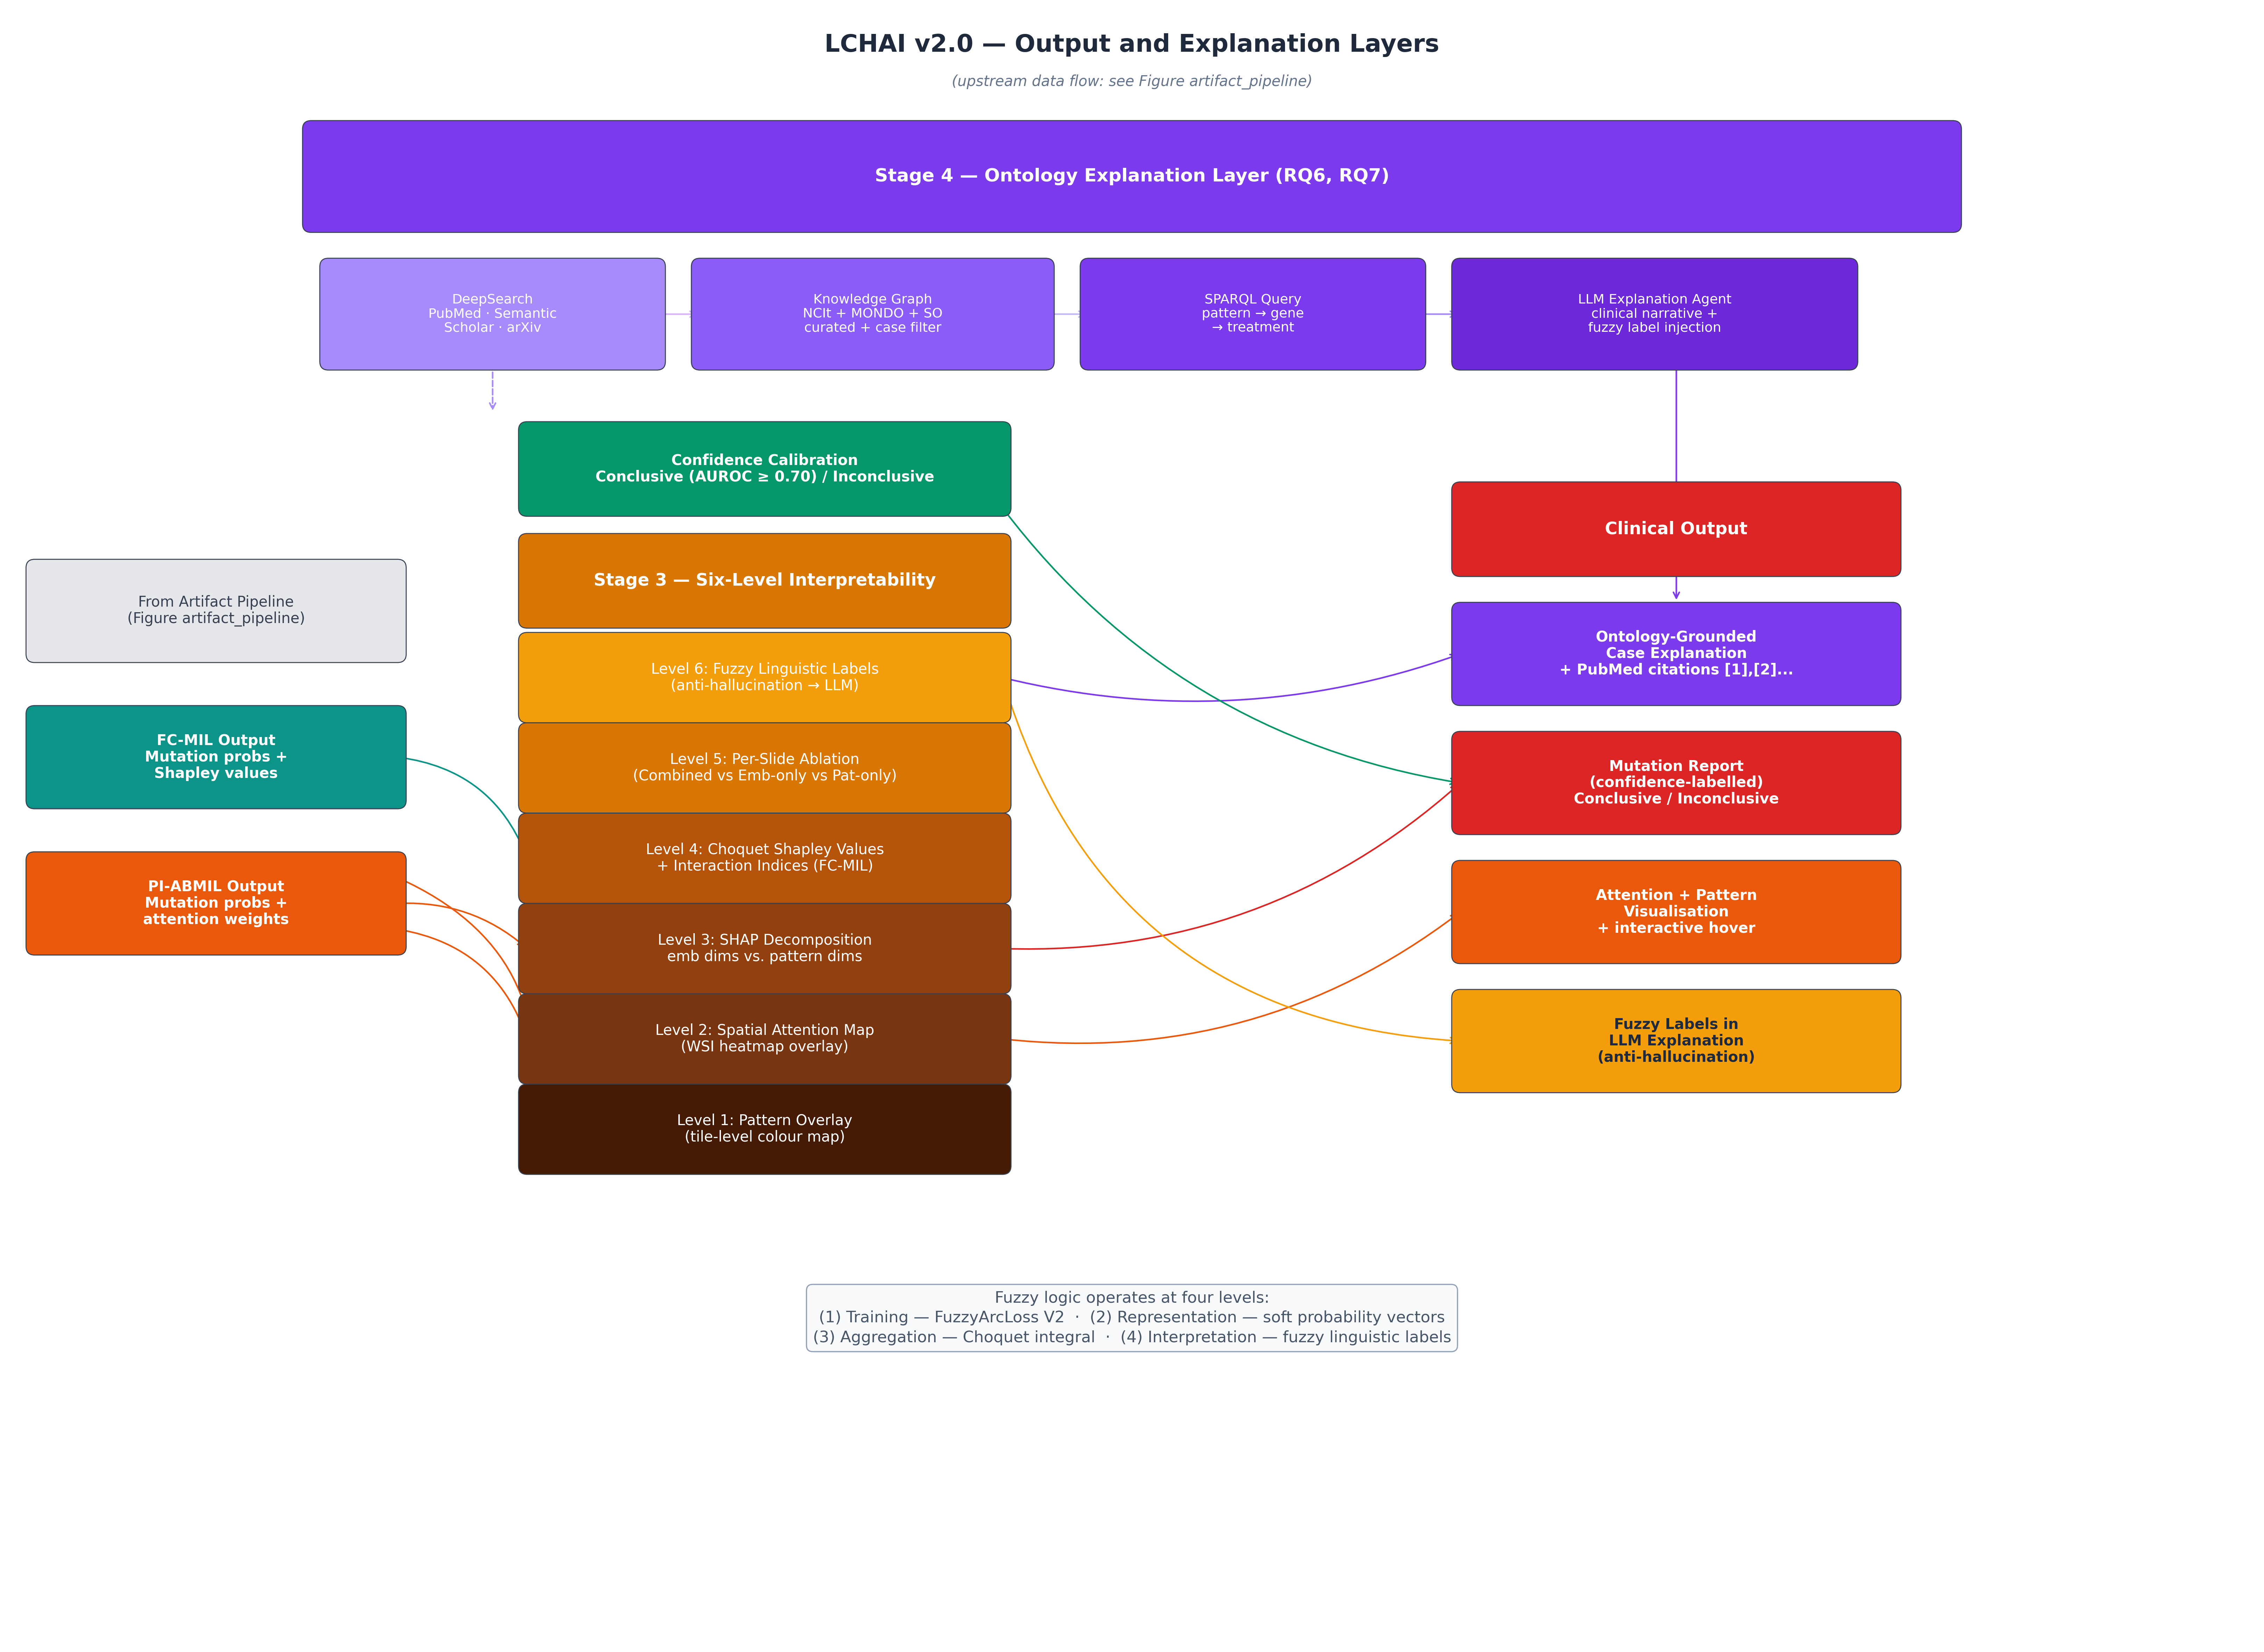
\includegraphics[width=\textwidth]{chapters/figures/lchai_v12_pipeline_new.png}
  \caption[LCHAI v2.0 output and explanation layers]{%
      LCHAI~v2.0 output and explanation layers, applied to the outputs
      of the three computational artefacts
      (see Figure~\ref{fig:artifact_pipeline_concept} for the upstream
      data flow).
      \emph{Left column (Interpretability, Stage~3):}
      Six levels following the canonical numbering of
      Chapter~\ref{ch:methodology},
      Section~\ref{sec:meth:interpretability}:
      (1)~spatial attention map, (2)~pattern attribution,
      (3)~SHAP decomposition, (4)~Choquet Shapley values (FC-MIL only),
      (5)~per-slide feature-channel ablation, and (6)~fuzzy linguistic
      labels injected into LLM explanations as anti-hallucination
      guardrails.
      All predictions carry a Conclusive/Inconclusive label.
      \emph{Right column (Clinical Output):}
      Ontology-grounded explanation with numbered PubMed citations,
      confidence-labelled mutation report, attention and pattern
      visualisation with interactive hover, and fuzzy-label-controlled
      LLM narrative (dual anti-hallucination).
      \emph{Top (Explanation layer, Stage~4, RQ6--RQ7):}
      DeepSearch pipeline (dashed arrow) periodically enriches the
      knowledge graph; edge store queries retrieve the pattern $\to$
      gene $\to$ treatment chain.}
  \label{fig:lchai_v12_pipeline}
\end{figure}

\textbf{Evaluation:}
LCHAI is evaluated as a system demonstration (DSR ``demonstration''
activity) rather than through a formal clinical trial.
The demonstration is conducted on representative TCGA-LUAD slides
using trained checkpoints from the benchmark run, using the LCHAI~v2.0 system.
Worked examples are presented in Section~\ref{sec:eval:lchai}.


\subsection{Summary: Artefact Pipeline}
\label{sec:uc:artifact_pipeline}

Figure~\ref{fig:artifact_pipeline_concept} illustrates the data flow
through the three artefacts, from raw WSI to slide-level mutation
predictions.

\textbf{Stage~1 (Preprocessing and Pattern Classification).}
Each WSI is partitioned into 5{,}000--80{,}000 tiles at $20\times$
magnification.
Tiles are passed through the CTransPath encoder (frozen after
fine-tuning) to produce 512-dimensional embeddings $\mathbf{x}_i$.
Artefact~1 (FuzzyArcLoss~V2 pattern classifier) generates a
6-dimensional fuzzy pattern probability vector
$\mathbf{p}_i \in \Delta^5$ for each tile, representing its degree of
membership in the six LUAD growth patterns.

\textbf{Stage~2 (Feature Fusion).}
The embedding and pattern probability vectors are concatenated to form
an enriched 518-dimensional tile representation:
$\mathbf{h}_i = [\mathbf{x}_i \,\|\, \mathbf{p}_i] \in
\mathbb{R}^{518}$.

\textbf{Stage~3 (Mutation Prediction).}
Two alternative aggregation architectures produce slide-level
mutation predictions, both operating on the same
$(\mathbf{x}_i, \mathbf{p}_i)$ inputs.
\emph{Artefact~2 (Pattern-Informed ABMIL)} applies gated attention
over the concatenated 518-d enriched representations $\mathbf{h}_i$.
\emph{Artefact~3 (Fuzzy Choquet MIL)} adopts a \emph{dual-pathway}
architecture: an ABMIL branch on the 512-d embeddings $\mathbf{x}_i$
runs in parallel with a learned Choquet integral over the 6-d
pattern memberships $\mathbf{p}_i$, and the two branch outputs are
merged before the final classification head
(Chapter~\ref{ch:methodology},
Section~\ref{sec:meth:choquet_mil}).
Both pathways feed into the LCHAI~v2.0 clinical decision-support
prototype (Section~\ref{sec:uc:lchai}).

\begin{figure}[ht!]
    \centering
    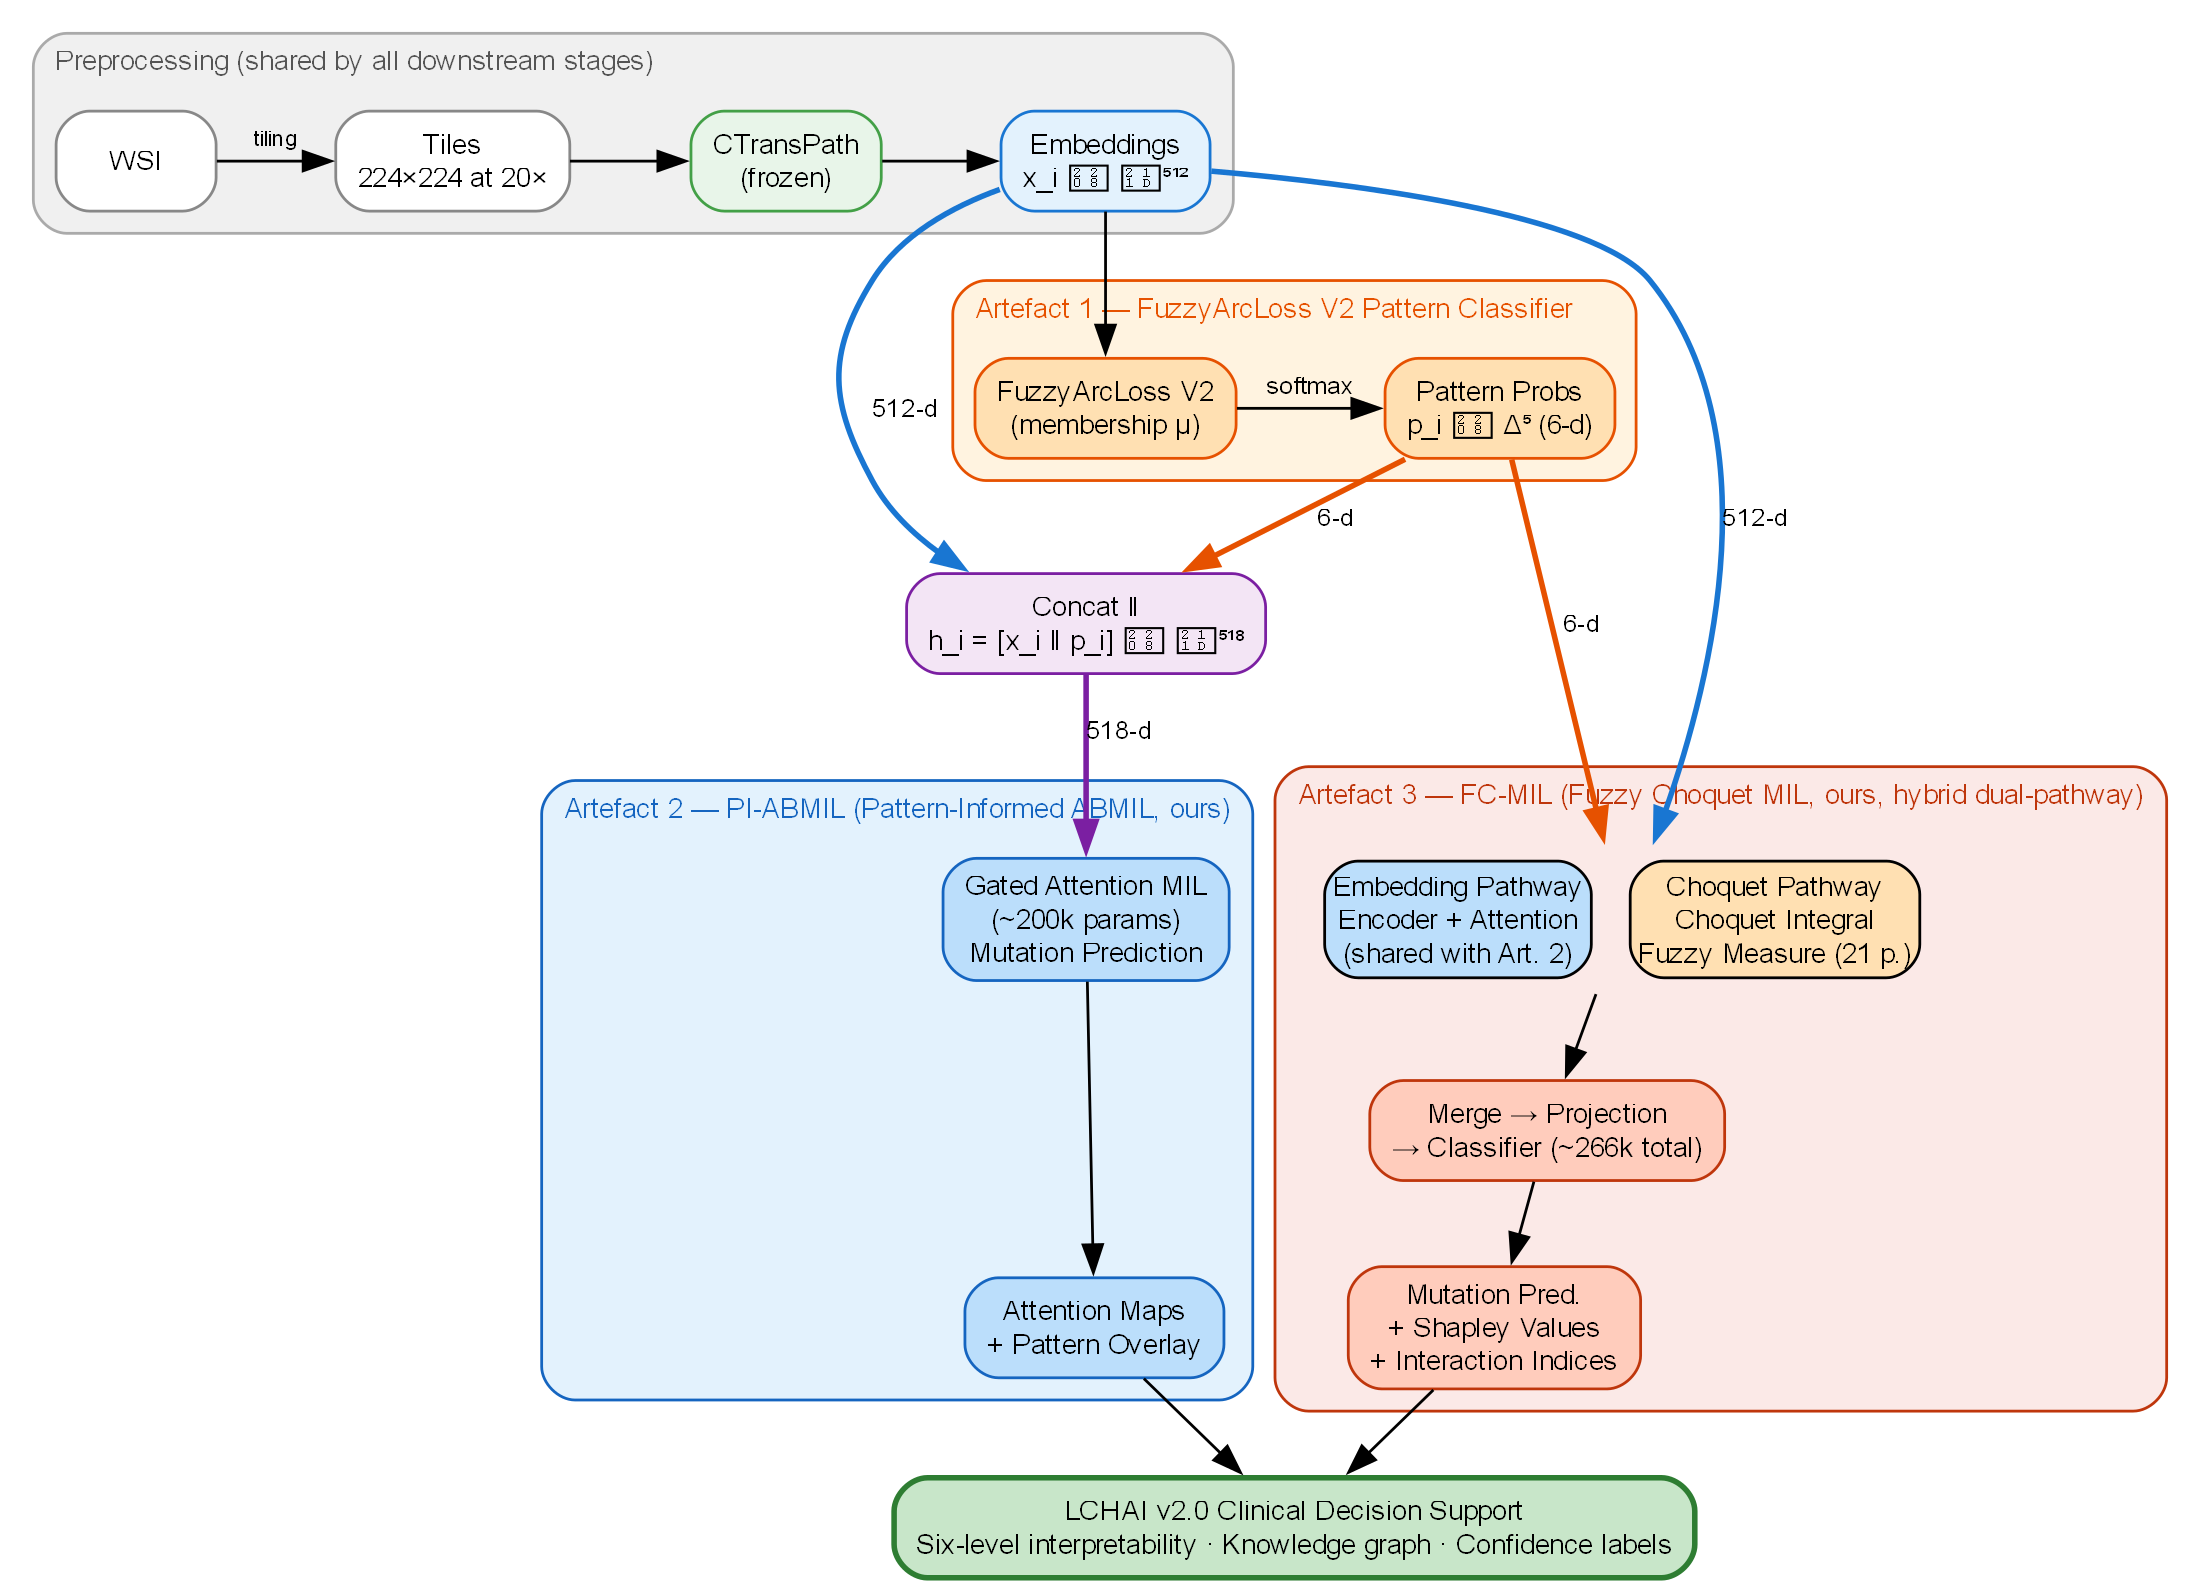
\includegraphics[width=\textwidth]{chapters/figures/artifact_pipeline.png}
    \caption[Conceptual pipeline linking the three computational
    artefacts]{%
        Conceptual data-flow pipeline linking the three computational
        artefacts.
        \emph{Solid arrows}: primary data flow from WSI through
        CTransPath embeddings, FuzzyArcLoss~V2 pattern probabilities,
        and feature concatenation to PI-ABMIL
        (Artefact~2, ours).
        \emph{Dashed arrow}: FC-MIL (Artefact~3, ours) receives the
        6-d pattern probability vectors $\mathbf{p}_i$ directly.
        In the implemented architecture, FC-MIL also receives the
        512-d embeddings through a shared encoder--attention pathway
        (solid arrow); the Choquet integral operates on the 6-d pattern
        vectors in a parallel branch, and both outputs are merged before
        classification.
        The preprocessing stage (grey box) is shared by all downstream
        conditions.
        The six pattern classes are: lepidic, acinar, papillary,
        micropapillary, solid, and cribriform.
        The LCHAI~v2.0 prototype (bottom) integrates both artefact
        outputs with a six-level interpretability framework, an ontology
        explanation layer, and Conclusive/Inconclusive confidence
        labels (Figure~\ref{fig:lchai_v12_pipeline}).}
    \label{fig:artifact_pipeline_concept}
\end{figure}


% ============================================================================
\section{Experimental Design: Headline}
\label{sec:uc:experimental_design}
% ============================================================================

The mutation prediction benchmark evaluates six experimental
conditions---XGBoost floor (B1), ABMIL on embeddings (B2), ABMIL on
patterns (B3), Pattern-Informed ABMIL (PI-ABMIL, ours), a crisp
one-hot ablation (A), and Fuzzy Choquet MIL (FC-MIL, ours)---under
5-fold patient-stratified cross-validation on the 687 LUAD slides
described above.
The formal definition of each condition's tile-level representation,
the ablation logic that maps each pairwise comparison to the research
questions of Section~\ref{sec:uc:clinical_questions}, and the
mathematical specification of the proposed methods are deferred to
Chapter~\ref{ch:methodology}
(Section~\ref{sec:meth:mutation_prediction} for the conditions and
Section~\ref{sec:meth:eval:ablation} for the ablation logic).
The empirical results, statistical tests, and per-gene mechanism
analysis are reported in Chapter~\ref{ch:evaluation}.


% ============================================================================
\section{Chapter Summary}
\label{sec:uc:summary}
% ============================================================================

This chapter has defined the cancer use case through eight components:

\begin{enumerate}
    \item \textbf{The clinical problem:} predicting somatic mutations
    from H\&E-stained whole-slide images to support treatment decisions
    when molecular profiling is slow or unavailable, with a requirement
    for explainability.

    \item \textbf{The histopathological domain:} six ANORAK-annotated
    LUAD growth patterns (five WHO-defined: lepidic, acinar, papillary,
    micropapillary, solid; plus the cribriform pattern) with detailed
    morphological descriptions, grading significance, and intra-tumoral
    heterogeneity.

    \item \textbf{The molecular landscape:} six target genes
    (\textit{TP53}, \textit{EGFR}, \textit{KRAS}, \textit{STK11},
    \textit{KEAP1}, \textit{RBM10}) consolidated in a single reference
    table (Table~\ref{tab:gene_unified}) that links each gene's
    prevalence, morphological correlate, biological mechanism, targeted
    therapy, and \emph{a priori} expected discrimination mode.

    \item \textbf{The datasets:} the Zenodo--ANORAK expert-annotated
    dataset (637 H\&E tile images, 6 pattern classes) for pattern
    classification, and the TCGA-LUAD cohort (687 whole-slide images
    from 668 patients, 6 target genes) for mutation prediction.

    \item \textbf{The data scarcity challenge:} publicly available LUAD
    data with both WSIs and mutation annotations is limited to
    $\sim$897 patients across all known cohorts (668 TCGA $+$ 229 from
    CPTAC-3, APOLLO, and EAGLE), two orders of magnitude below the
    proprietary datasets used by state-of-the-art methods.
    This gap motivates methodological innovation over scale competition.

    \item \textbf{The research-question mapping and artefact vision:}
    a use-case-specific mapping (Table~\ref{tab:rq_mapping}) of the
    seven research questions of
    Chapter~\ref{ch:introduction} (RQ1--RQ7, including the
    decomposition of RQ2 into RQ2(i)/(ii)) onto three computational
    artefacts and the LCHAI~v2.0 clinical decision support prototype.

    \item \textbf{Pipeline audit headline:} a systematic audit of the
    pattern-classification training pipeline raised macro-F1
    \emph{uniformly across all 18 loss-function variants} by
    approximately 18~percentage points
    ($\sim 71$--$76\,\% \to 89$--$95\,\%$),
    establishing a fair shared baseline rather than preferentially
    advantaging any one method;
    the methodologically significant fixes are detailed in
    Chapter~\ref{ch:methodology}
    (Section~\ref{sec:meth:pattern:pipeline_audit}).

    \item \textbf{Experimental design headline:} a six-condition
    benchmark (B1~XGBoost, B2~ABMIL-embeddings, B3~ABMIL-patterns,
    PI-ABMIL~(ours), A~one-hot ablation, FC-MIL~(ours)) under 5-fold
    patient-stratified cross-validation; the formal ablation logic
    that maps each pairwise comparison to a research question is in
    Chapter~\ref{ch:methodology}, Section~\ref{sec:meth:eval:ablation}.
\end{enumerate}

The following chapter (Chapter~\ref{ch:methodology}) details the design
and mathematical formulation of each artefact, while
Chapter~\ref{ch:implementation} describes their implementation and
Chapter~\ref{ch:evaluation} presents the evaluation results.
